\documentclass{report}
% Verilog code formatting ref: https://tex.stackexchange.com/questions/377122/typesetting-for-a-verilog-lstinput
\usepackage{xcolor}
\usepackage{listings}
\definecolor{vgreen}{RGB}{104,180,104}
\definecolor{vblue}{RGB}{49,49,255}
\definecolor{vorange}{RGB}{255,143,102}

\lstdefinestyle{verilog-style}
{
    language=Verilog,    
    breaklines=true,    
    basicstyle=\small\ttfamily,
    keywordstyle=\color{vblue},
    identifierstyle=\color{black},
    commentstyle=\color{vgreen},
    numbers=left,
    numberstyle=\tiny\color{black},
    numbersep=10pt,
    tabsize=8,
    moredelim=*[s][\colorIndex]{[}{]},
    literate=*{:}{:}1
}

\definecolor{mGreen}{rgb}{0,0.6,0}
\definecolor{mGray}{rgb}{0.5,0.5,0.5}
\definecolor{mPurple}{rgb}{0.58,0,0.82}
\definecolor{backgroundColour}{rgb}{0.95,0.95,0.92}

\lstdefinestyle{CStyle}{
    backgroundcolor=\color{backgroundColour},   
    commentstyle=\color{mGreen},
    keywordstyle=\color{magenta},
    numberstyle=\tiny\color{mGray},
    stringstyle=\color{mPurple},
    basicstyle=\footnotesize,
    breakatwhitespace=false,         
    breaklines=true,                 
    captionpos=b,                    
    keepspaces=true,                 
    numbers=left,                    
    numbersep=5pt,                  
    showspaces=false,                
    showstringspaces=false,
    showtabs=false,                  
    tabsize=2,
    language=C
}

\makeatletter
\newcommand*\@lbracket{[}
\newcommand*\@rbracket{]}
\newcommand*\@colon{:}
\newcommand*\colorIndex{%
    \edef\@temp{\the\lst@token}%
    \ifx\@temp\@lbracket \color{black}%
    \else\ifx\@temp\@rbracket \color{black}%
    \else\ifx\@temp\@colon \color{black}%
    \else \color{vorange}%
    \fi\fi\fi
}
\makeatother
\usepackage{trace}

\setcounter{secnumdepth}{3} % To add subsubsections to the table of contents
% for QnA ref: https://latex.org/forum/viewtopic.php?t=10494
\newcounter{question}
\setcounter{question}{0}
\newcommand{\question}[1]{\item[\textbf{Q\refstepcounter{question}\thequestion.}] \textbf{#1}}
\newcommand{\answer}[1]{\item[Answer:] #1}


% A pretty common set of packages
\usepackage[margin=2.5cm]{geometry}
\usepackage[T1]{fontenc}
\usepackage[utf8]{inputenc}
\usepackage{blindtext}
\author{Maitreya Ranade}
\date{\today}
\usepackage{pdfpages}
\usepackage{graphicx}
\usepackage{amssymb}
\usepackage{amsmath}
\usepackage{color}
\usepackage{import}
\usepackage{booktabs}
\usepackage{multirow}
\usepackage{engord}
\usepackage{soul}
\usepackage{textcomp}
\usepackage{parskip}
\usepackage{setspace}
\usepackage{titlesec}
\usepackage{fancyhdr}
\usepackage{tabularx}
\usepackage{mathtools} % for '\DeclarePairedDelimiter' macro
\DeclarePairedDelimiter\norm\lVert\rVert
\usepackage{bookmark}
\pagestyle{fancy}
\usepackage[UKenglish]{babel}
\usepackage[UKenglish]{isodate}
\usepackage[skip=2pt,font=footnotesize,justification=centering]{caption}
\usepackage{natbib}
\usepackage{float}
\usepackage{dirtree}
\usepackage{url}
\usepackage{enumitem}
\usepackage{tgpagella}


% Custom environments
\newenvironment{highlight}
{\vspace{2mm} \hrule \vspace{2mm} \em}
{\vspace{2mm} \hrule \vspace{2mm}}


% Make some additional useful commands
\newcommand{\ie}{\emph{i.e.}\ }
\newcommand{\eg}{\emph{e.g.}\ }
\newcommand{\etal}{\emph{et al}}
\newcommand{\sub}[1]{$_{\textrm{#1}}$}
\newcommand{\super}[1]{$^{\textrm{#1}}$}
\newcommand{\degC}{$^{\circ}$C}
\newcommand{\wig}{$\sim$}
\newcommand{\ord}[1]{\engordnumber{#1}}
\newcommand{\num}[2]{$#1\,$#2}
\newcommand{\range}[3]{$#1$-$#2\,$#3}
\newcommand{\roughly}[2]{$\sim\!#1\,$#2}
\newcommand{\area}[3]{$#1 \! \times \! #2\,$#3}
\newcommand{\vol}[4]{$#1 \! \times \! #2 \! \times \! #3\,$#4}
\newcommand{\cube}[1]{$#1 \! \times \! #1 \! \times \! #1$}
\newcommand{\figref}[1]{Figure~\ref{#1}}
\newcommand{\eqnref}[1]{Equation~\ref{#1}}
\newcommand{\tableref}[1]{Table~\ref{#1}}
\newcommand{\secref}[1]{Section \ref{#1}}
\newcommand{\XC}{\emph{exchange-correlation}}
\newcommand{\abinit}{\emph{ab initio}}
\newcommand{\Abinit}{\emph{Ab initio}}
\newcommand{\Lonetwo}{L1$_{2}$}
\newcommand{\Dznt}{D0$_{19}$}
\newcommand{\Dtf}{D8$_{5}$}
\newcommand{\Btwo}{B$_{2}$}
\newcommand{\fcc}{\emph{fcc}}
\newcommand{\hcp}{\emph{hcp}}
\newcommand{\bcc}{\emph{bcc}}
\newcommand{\Ang}{{\AA}}
\newcommand{\inverseAng}{{\AA}$^{-1}$}
\newcommand{\comment}[1]{\textcolor{red}{[COMMENT: #1]}}
\newcommand{\more}{\textcolor{red}{[MORE]}}
\newcommand{\red}[1]{\textcolor{red}{#1}}
\newcommand{\SubItem}[1]{
    {\setlength\itemindent{15pt} \item[] \textbf{#1}}
}
% Change this to modify look of header and footer
\lhead{}
\chead{}
\rhead{}
\lfoot{}
\cfoot{\thepage{}}
\rfoot{}
\renewcommand{\headrulewidth}{0pt}
\renewcommand{\footrulewidth}{0pt}
\usepackage{hyperref}
\hypersetup{
    colorlinks=true,
    linkcolor=blue,
    filecolor=magenta,      
    urlcolor=cyan,
}
\urlstyle{same}
\newcommand{\foo}{\hspace{-2.3pt}$\bullet$ \hspace{5pt}}   % For timeline
  

\begin{document}
	\onehalfspacing
	Date: \today{} \hfill{} Name: Maitreya Ranade
	\begin{center}
		\topskip0pt
		\vspace*{\fill}
		{\LARGE High-Level Synthesis} \\
		This report is written for personal understanding and not for publication or distribution.
		\vspace*{\fill}
	\end{center}
	
	\pagebreak
	\singlespacing
	\tableofcontents
	\pagebreak       

  \chapter{High-Level Synthesis Prerequisites}   
  \section{Introduction}
Software is the basis of all applications. Based on the performance and programmability constraints of the
system, the software engineer is tasked with determining the best implementation platform
to get a project to market. To accomplish this task, the software engineer is aided by both
programming techniques and a variety of hardware processing platforms.

\par On the programming side, previous decades yielded advances in object-oriented
programming for code reuse and parallel computing paradigms for boosting algorithm
performance. The advancements in programming languages, frameworks, and tools
allowed the software engineer to quickly prototype and test different approaches to solve
a particular problem.

\par Although the interest in the parallel and concurrent execution of software
programs is not new, the renewed and increased interest is aided by certain trends in
processor and application-specific integrated circuit (ASIC) design. There are two crucial 
factors for getting more performance out of a software algorithm  with the use of a
custom-integrated circuit or an FPGA:
\begin{itemize}
  \item Cost to fabricate the circuit
  \item Time to translate the algorithm into hardware 
\end{itemize}

Despite advancements in fabrication process node technology that have yielded significant
improvements in power consumption, computational throughput, and logic density, the
cost to fabricate a custom-integrated circuit or ASIC for an application is still high. At each
processing node, the cost of fabrication continues to increase to the point where this
approach is only economically viable for applications that ship in the range of millions of
units.

\par The second option is to use an FPGA, which addresses the cost issues inherent in ASIC
fabrication. FPGAs allow the designer to create a custom circuit implementation of an
algorithm using an off-the-shelf component composed of basic programmable logic
elements. This platform offers the power consumption savings and performance benefits of
smaller fabrication nodes without incurring the cost and complexity of an ASIC
development effort. Similar to an ASIC, an algorithm implemented in an FPGA benefits from
the inherent parallel nature of a custom circuit.

\clearpage
\subsection{Programming Model}

The programming model of a hardware platform is one of the driving factors behind its adoption. Software algorithms are typically captured in C/C++ or some other high-level
language, which abstracts the details of the computing platform. These languages allow for
quick iteration, incremental improvements, and code portability, which are critical to the
software engineer.

\par With the recent paradigm shift in the design of standard and specialized processors, both
types of processors stopped relying on clock frequency increases for program speedup and
added more processing cores per chip. Multicore processors put program parallelization at
the forefront of techniques used to boost software performance. The software engineer
must now structure algorithms in a way that leads to efficient parallelization for
performance. The techniques required in algorithm design use the same base elements of
FPGA design. The main difference between an FPGA and a processor is the programming
model.

\par Historically, the programming model of an FPGA was centered on register-transfer level
(RTL) descriptions instead of C/C++. Although this model of design capture is completely
compatible with ASIC design, it is analogous to assembly language programming in
software engineering. 

\par Both the initial and optimized versions of an application with an
FPGA platform provide significant performance when compared against the same 
stages for both standard and specialized
processors. RTL coding and an FPGA optimized application result in the highest
performance implementation. However, the development time required to arrive at this implementation is beyond the
scope of a typical software development effort. Therefore, FPGAs were traditionally used
only for those applications requiring a performance profile that could not be achieved by
any other means, such as designs with multiple processors.

\par Recent technological advances by Xilinx remove the difference in programming models
between a processor and an FPGA. Just as there are compilers from C and other high-level
languages to different processor architectures, the Xilinx Vivado High-Level Synthesis
(HLS) compiler provides the same functionality for C/C++ programs targeted to Xilinx
FPGAs.

\clearpage
\section{FPGA Architecture}   
An FPGA is a type of integrated circuit (IC) that can be programmed for different algorithms
after fabrication. Modern FPGA devices consist of up to two million logic cells that can be
configured to implement a variety of software algorithms. Although the traditional FPGA
design flow is more similar to a regular IC than a processor, an FPGA provides significant
cost advantages in comparison to an IC development effort and offers the same level of
performance in most cases. Another advantage of the FPGA when compared to the IC is its
ability to be dynamically reconfigured. This process, which is the same as loading a program
in a processor, can affect part or all of the resources available in the FPGA fabric.

\par The basic structure of an FPGA is composed of the following elements:
\begin{itemize}
  \item Look-up table (LUT): This element performs logic operations.
  \item Flip-Flop (FF): This register element stores the result of the LUT.
  \item Wires: These elements connect elements to one another.
  \item Input/Output (I/O) pads: These physically available ports get data in and out of the FPGA.
\end{itemize}

The combination of these elements results in the basic FPGA architecture shown in \figref{FPGAArch}. 
Although this structure is sufficient for the implementation of any algorithm,
the efficiency of the resulting implementation is limited in terms of computational
throughput, required resources, and achievable clock frequency.

\begin{figure}[H]
  \begin{center}
      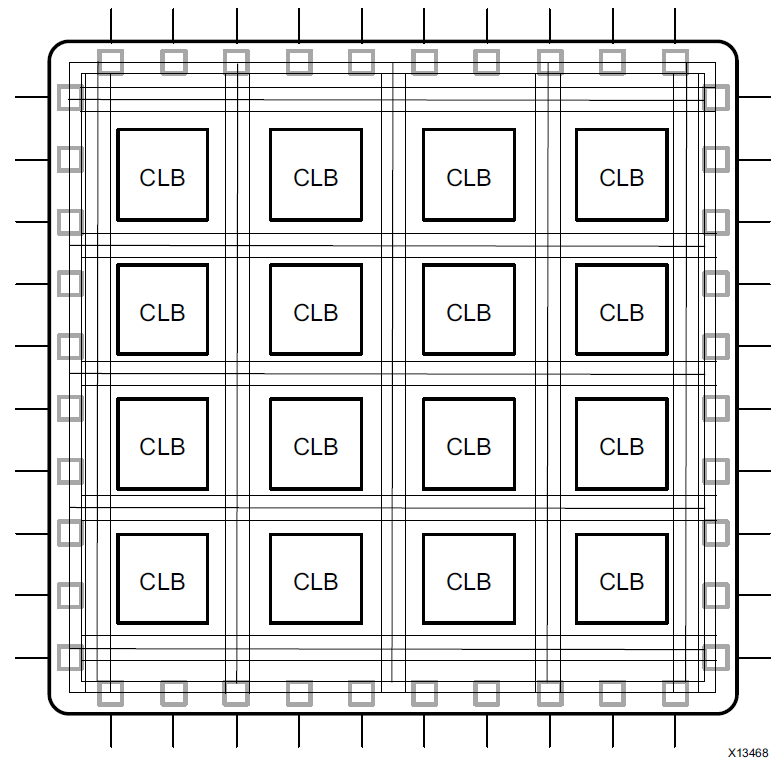
\includegraphics[width=0.75\textwidth]{images/FPGAArch.png}
      \caption{Basic FPGA Architecture}
      \label{FPGAArch}
  \end{center}
\end{figure}

\clearpage


Contemporary FPGA architectures incorporate the basic elements along with additional
computational and data storage blocks that increase the computational density and
efficiency of the device. These additional elements are:
\begin{itemize}
  \item Embedded memories for distributed data storage
  \item Phase-locked loops (PLLs) for driving the FPGA fabric at different clock rates
  \item High-speed serial transceivers
  \item Off-chip memory controllers
  \item Multiply-accumulate blocks
\end{itemize}

The combination of these elements provides the FPGA with the flexibility to implement any
software algorithm running on a processor and results in the contemporary FPGA architecture shown in \figref{ContempFPGAArch}.

\begin{figure}[H]
  \begin{center}
      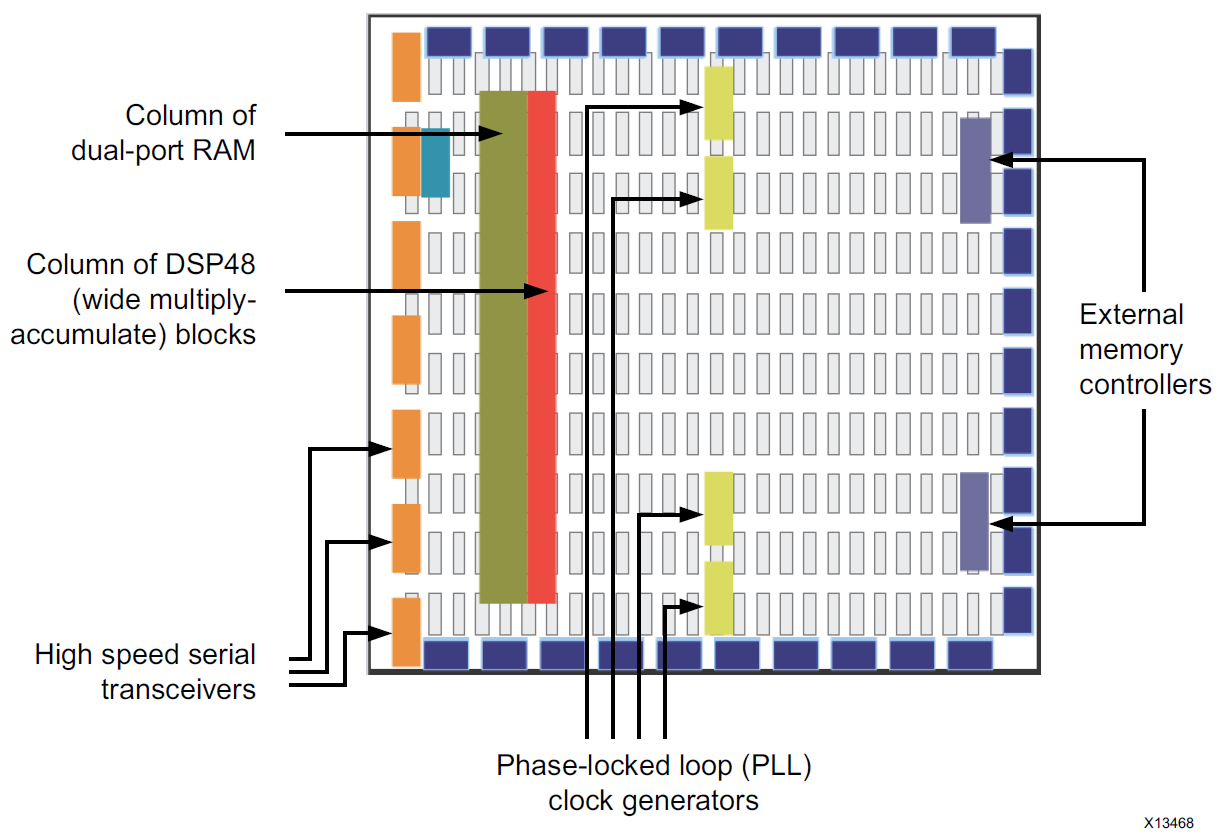
\includegraphics[width=\textwidth]{images/ContempFPGAArch.png}
      \caption{Contemporary FPGA Architecture}
      \label{ContempFPGAArch}
  \end{center}
\end{figure}

\clearpage
\subsection{Look Up Table (LUT)}
The LUT is the basic building block of an FPGA and is capable of implementing any logic
function of N Boolean variables. Essentially, this element is a truth table in which different
combinations of the inputs implement different functions to yield output values. The limit
on the size of the truth table is N, where N represents the number of inputs to the LUT. For
the general N-input LUT, the number of memory locations accessed by the table is:
\[ 2^{N} \]
which allows the table to implement the following number of functions:
\[ 2^{N^{N}} \]

\begin{highlight}
  Note: A typical value for N in Xilinx FPGA devices is 6.  
\end{highlight}

The hardware implementation of a LUT can be thought of as a collection of memory cells
connected to a set of multiplexers. The inputs to the LUT act as selector bits on the
multiplexer to select the result at a given point in time. It is important to keep this
representation in mind, because a LUT can be used as both a function compute engine and
a data storage element. \figref{LUT} shows this functional representation of the LUT.

\begin{figure}[H]
  \begin{center}
      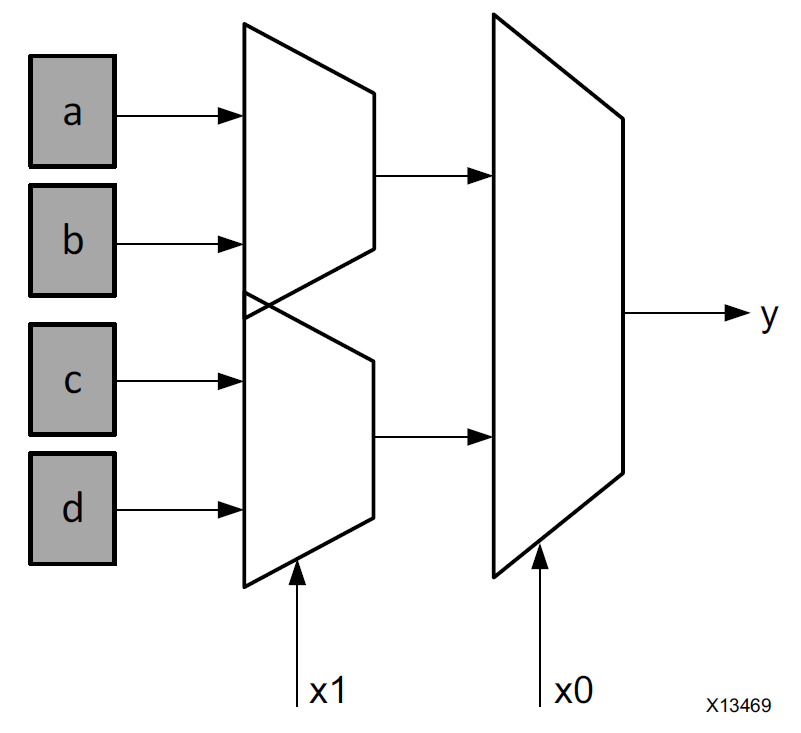
\includegraphics[width=0.6\textwidth]{images/LUT.png}
      \caption{Functional Representation of a LUT as Collection of Memory Cells}
      \label{LUT}
  \end{center}
\end{figure}

\clearpage

\subsection{Flip-Flop}

The flip-flop is the basic storage unit within the FPGA fabric. This element is always paired
with a LUT to assist in logic pipelining and data storage. The basic structure of a flip-flop
includes a data input, clock input, clock enable, reset, and data output. During normal
operation, any value at the data input port is latched and passed to the output on every
pulse of the clock. The purpose of the clock enable pin is to allow the flip-flop to hold a
specific value for more than one clock pulse. New data inputs are only latched and passed
to the data output port when both clock and clock enable are equal to one. \figref{flipflop}
shows the structure of a flip-flop.

\begin{figure}[H]
  \begin{center}
      \includegraphics[width=0.4\textwidth]{images/flipflop.png}
      \caption{Structure of a Flip-Flop}
      \label{flipflop}
  \end{center}
\end{figure}
\clearpage

\subsection{DSP Block}
The most complex computational block available in a Xilinx FPGA is the DSP block, which is
shown in \figref{dsp}. The DSP block is an arithmetic logic unit (ALU) embedded into the
fabric of the FPGA, which is composed of a chain of three different blocks. The
computational chain in the DSP is composed of an add/subtract unit connected to a
multiplier connected to a final add/subtract/accumulate engine. This chain allows a single
DSP unit to implement functions of the form:
\[ p \: =\: a*( b + d) + c\] 
or
\[ p \: +=\: a*( b + d) \] 

\begin{figure}[H]
  \begin{center}
      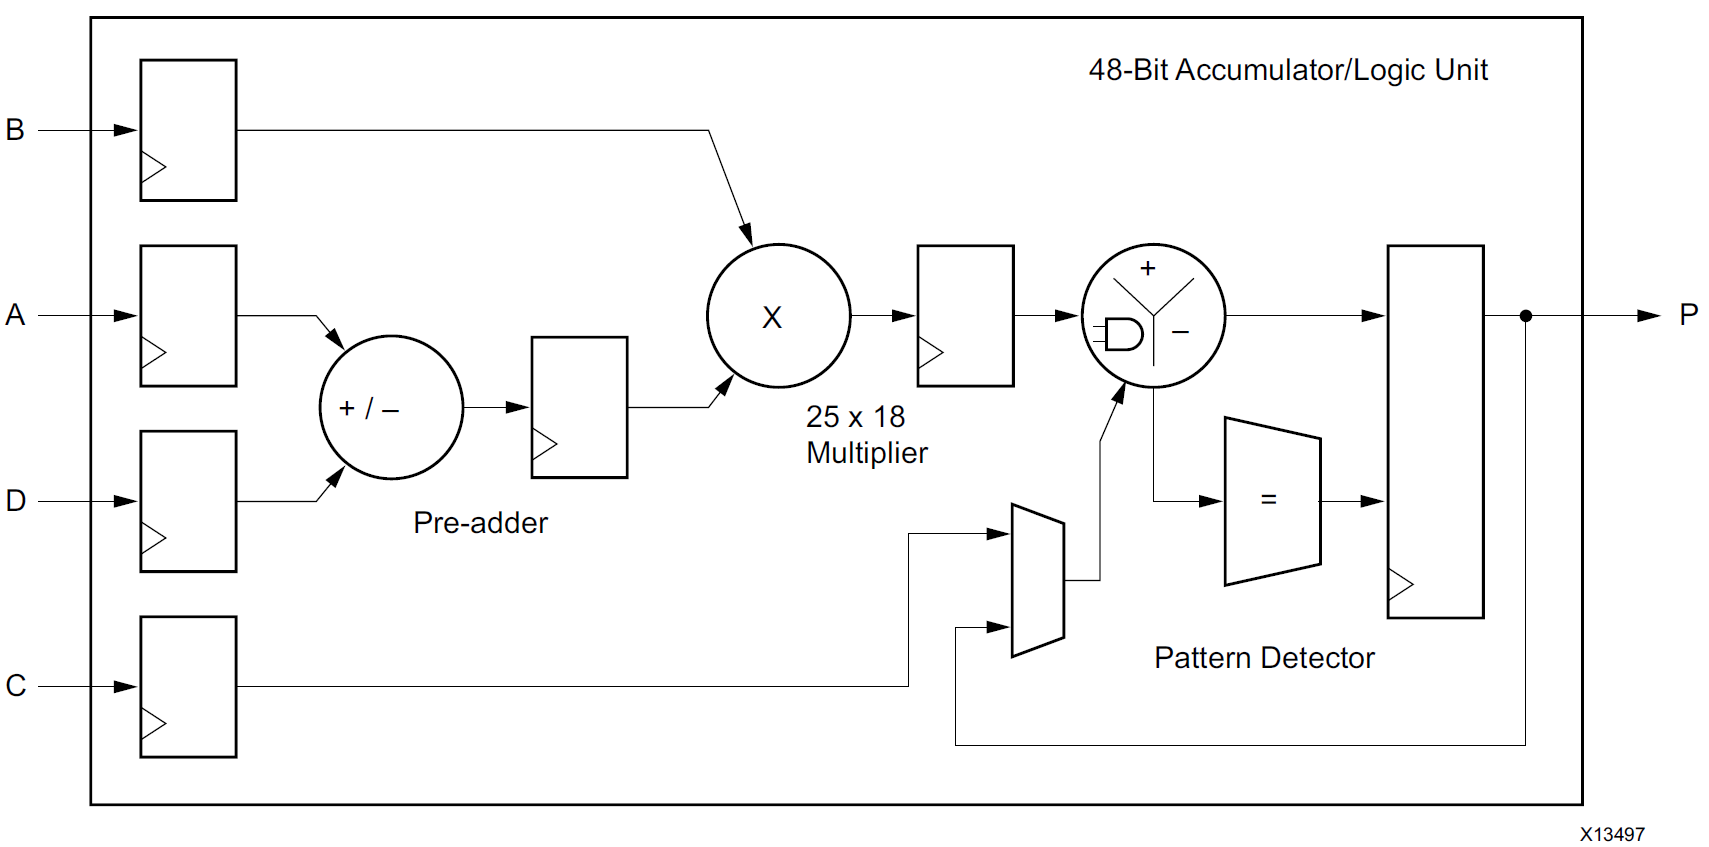
\includegraphics[width=\textwidth]{images/dsp.png}
      \caption{Structure of a DSP Block}
      \label{dsp}
  \end{center}
\end{figure}

\clearpage
\subsection{Storage Elements}
The FPGA device includes embedded memory elements that can be used as random-access memory (RAM), read-only memory (ROM), or shift registers. These elements are:

\begin{enumerate}
  \item Block RAMs (BRAMs), 
  \item UltraRAM blocks (URAMS),
  \item LUTs, and 
  \item Shift registers (SRLs).
\end{enumerate} 

\subsubsection{BRAM}
The BRAM is a dual-port RAM module instantiated into the FPGA fabric to provide on-chip storage for a relatively large set of data. The two types of BRAM memories available in a
device can hold either 18k or 36k bits. The number of these memories available is device
specific. The dual-port nature of these memories allows for parallel, same-clock-cycle
access to different locations.
In terms of how arrays are represented in C/C++ code, BRAMs can implement either a RAM
or a ROM. The only difference is when the data is written to the storage element. In a RAM configuration, the data can be read and written at any time during the runtime of the
circuit. In contrast, in a ROM configuration, data can only be read during the runtime of the
circuit. The data of the ROM is written as part of the FPGA configuration and cannot be
modified in any way.

\subsubsection{URAM}
The UltraRAM blocks are dual-port, synchronous 288 Kb RAM with a fixed configuration of
4,096 bits deep and 72 bits wide. They are available on UltraScale+ Devices and provide 8
times more storage capacity than the BRAM.

\subsubsection{LUT}
As previously discussed, the LUT is a small memory in which the contents of a truth table are
written during device configuration. Due to the flexibility of the LUT structure in Xilinx
FPGAs, these blocks can be used as 64-bit memories and are commonly referred to as
distributed memories. This is the fastest kind of memory available on the FPGA device,
because it can be instantiated in any part of the fabric that improves the performance of the
implemented circuit.

\subsubsection{Shift Register}
The shift register is a chain of registers connected to each other. The purpose of this
structure is to provide data reuse along a computational path. 


\clearpage
\section{FPGA Parallelism Versus Processor Architectures}
When compared with processor architectures, the structures that comprise the FPGA fabric
enable a high degree of parallelism in application execution. The custom processing
architecture generated by the Vivado HLS compiler for a software program presents a
different execution paradigm, which must be taken into account when deciding to port an
application from a processor to an FPGA. 

\subsection{Program Execution on a Processor}
A processor, regardless of its type, executes a program as a sequence of instructions that
translate into useful computations for the software application. This sequence of
instructions is generated by processor compiler tools, such as the GNU Compiler Collection
(GCC), which transform an algorithm expressed in C/C++ into assembly language
constructs that are native to the processor. 

\par Any assembly code can show that even a simple operation, results in multiple assembly instructions. 
The computational latency of each instruction is not equal across instruction types. 

\begin{highlight}
  IMPORTANT: The level of effort required by the software engineer in restructuring algorithms to better fit the available processor cache is not required when the same operation is implemented in an FPGA.
\end{highlight}

\subsection{Program Execution on an FPGA}
The FPGA is an inherently parallel processing fabric capable of implementing any logical
and arithmetic function that can run on a processor. The main difference is that the Vivado
HLS compiler, which is used to transform software descriptions into RTL, is not hindered by
the restrictions of a cache and a unified memory space. Every code is compiled by Vivado HLS into several LUTs required to achieve the
size of the output operand.

\begin{highlight}
  NOTE: As a general rule, 1 LUT is equivalent to 1 bit of computation.
\end{highlight}

LUTs used for a computation of a value are exclusive to that particular operation only. Unlike a
processor, where all computations share the same ALU, an FPGA implementation
instantiates independent sets of LUTs for each computation in the software algorithm. 

\par In addition to assigning unique LUT resources per computation, the FPGA differs from a
processor in both memory architecture and the cost of memory accesses. In an FPGA
implementation, the Vivado HLS compiler arranges memories into multiple storage banks
as close as possible to the point of use in the operation. This results in an instantaneous
memory bandwidth, which far exceeds the capabilities of a processor. 

\par With regard to computational throughput and memory bandwidth, the Vivado HLS
compiler exercises the capabilities of the FPGA fabric through the processes of scheduling,
pipelining, and dataflow. Although transparent to the user, these processes are integral
stages of the software compilation process that extract the best possible circuit-level
implementation of the software application.

\subsubsection{Scheduling}
Scheduling is the process of identifying the data and control dependencies between
different operations to determine when each will execute. Vivado HLS analyzes dependencies between adjacent operations as well as across time. This
allows the compiler to group operations to execute in the same clock cycle and to set up the
hardware to allow the overlap of function calls. The overlap of function call executions
removes the processor restriction that requires the current function call to fully complete
before the next function call to the same set of operations can begin. This process is called
pipelining.

\subsubsection{Pipelining}
Pipelining is a digital design technique that allows the designer to avoid data dependencies
and increase the level of parallelism in an algorithm hardware implementation. The data
dependence in the original software implementation is preserved for functional
equivalence, but the required circuit is divided into a chain of independent stages. All
stages in the chain run in parallel on the same clock cycle. The only difference is the source
of data for each stage. Each stage in the computation receives its data values from the result
computed by the preceding stage during the previous clock cycle. 

\subsubsection{Dataflow}
Dataflow is another digital design technique, which is similar in concept to pipelining. The
goal of dataflow is to express parallelism at a coarse-grain level. In terms of software
execution, this transformation applies to parallel execution of functions within a single
program. 

\par Vivado HLS extracts this level of parallelism by evaluating the interactions between different
functions of a program based on their inputs and outputs. The simplest case of parallelism
is when functions work on different data sets and do not communicate with each other. In
this case, Vivado HLS allocates FPGA logic resources for each function and then runs the blocks independently. The more complex case, which is typical in software programs, is when one function provides results for another function. This case is referred to as the consumer-producer scenario. Vivado HLS supports two use models for the consumer-producer scenario: 

\begin{itemize}
  \item In the first use
  model, the producer creates a complete data set before the consumer can start its
  operation. Parallelism is achieved by instantiating a pair of BRAM memories arranged as
  memory banks ping and pong. Each function can access only one memory bank, ping or
  pong, for the duration of a function call. When a new function call begins, the
  HLS-generated circuit switches the memory connections for both the producer and the
  consumer. This approach guarantees functional correctness but limits the level of
  achievable parallelism to across function calls.
  \item In the second use model, the consumer can start working with partial results from the
  producer, and the achievable level of parallelism is extended to include execution within a
  function call. The Vivado HLS-generated modules for both functions are connected through
  the use of a first in, first out (FIFO) memory circuit. This memory circuit, which acts as a
  queue in software programming, provides data-level synchronization between the modules.
  At any point during a function call, both hardware modules are executing their
  programming. The only exception is that the consumer module waits for some data to be
  available from the producer before beginning computation. In Vivado HLS terminology, the
  wait time of the consumer module is referred to as the interval or initiation interval (II).
\end{itemize}
\clearpage

\section{Basic Concepts of Hardware Design}

\textbf{One of the key differences between a processor and an FPGA is whether the processing
architecture is fixed.}

\par With a processor, the computation architecture is fixed, and the job of the compiler is to
determine how to best fit the software application in the available processing structures. Performance is a function of how well the application maps to the capabilities of the
processor and the number of processor instructions needed for correct execution.

\par In contrast, an FPGA is similar to a blank slate with a box of building blocks with the processing architecture not fixed. The job of the Vivado HLS compiler is to create a processing architecture from the box of building blocks that best fits the software program. The process of guiding the Vivado HLS compiler to
create the best processing architecture requires fundamental knowledge about hardware design concepts. As with processor compilers, the Vivado HLS compiler handles the
low-level details of the algorithm implementation into the FPGA logic fabric.

\subsection{Clock Frequency}

The processor clock frequency is one of the first items to consider when determining the
execution platform of a specific algorithm. A commonly used guideline is that a high clock
frequency translates into a higher performance execution rate of an algorithm. Although
this might be a good first order rule for choosing between processors, it is actually
misleading and can lead the designer to make the wrong choice when selecting between a
processor and an FPGA.

\subsubsection{Instruction execution}
The first major difference between a processor and an FPGA is how a software program is
executed. A processor is able to execute any program on a common hardware platform. This
common platform comprises the core of the processor and defines a fixed architecture onto
which all software must be fitted. The compiler, which has a built-in understanding of the
processor architecture, compiles the user software into a set of instructions. 

\par Regardless of the type of processor, standard versus specialized, the execution of an
instruction is always the same. Each instruction of the user application must go through the
following stages:
\begin{enumerate}
  \item Instruction fetch (IF)
  \item Instruction decode (ID)
  \item Execute (EXE)
  \item Memory operations (MEM)
  \item Write back (WB)
\end{enumerate}
The purpose of each stage is summarized below.
\begin{table}[H]
  \begin{tabular}{|p{0.1\linewidth} | p{0.85\linewidth}|}
  \hline
  \textbf{Stage} & \textbf{Description}                                                               \\ \hline
  IF             & Get the instruction from program memory.                                           \\ \hline
  ID             & Decode the instruction to determine the operation and the operators.             \\ \hline
  EXE            & Execute the instruction on the available hardware. In a standard processor, this means the arithmetic logic unit (ALU) or floating point unit (FPU). A specialized processor adds on fixed function accelerators to the capabilities of the standard processor at this stage of instruction processing. \\ \hline
  MEM            & Fetch data for the next instruction using memory operations.                     \\ \hline
  WB             & Write the results of the instruction either to local registers or global memory. \\ \hline
  \end{tabular}
\end{table}

Most modern processors include multiple copies of the instruction execution path and are
capable of running instructions with some degree of overlap. Because instructions in a
processor usually depend on each other, the overlap between copies of the instruction
execution hardware is not perfect. In the best of cases, only the overhead stages introduced
by using a processor can be overlapped. The EXE stages, which are responsible for
application computation, execute sequentially. The reasons for this sequential execution are
related to limited resources in the EXE stage and dependence between instructions.

\par \figref{multiProcessor} shows a processor with multiple instructions executing in a semi-parallel order.
This is the best case for a processor in which all instructions are executing as quickly as
possible. Even in this best case, the processor is limited to only one EXE stage per clock
cycle. This means that the user application moves forward by one operation per clock cycle.
Even if the compiler determined that all five EXE stages could execute in parallel, the
structure of the process would prevent it.

\begin{figure}[H]
  \begin{center}
      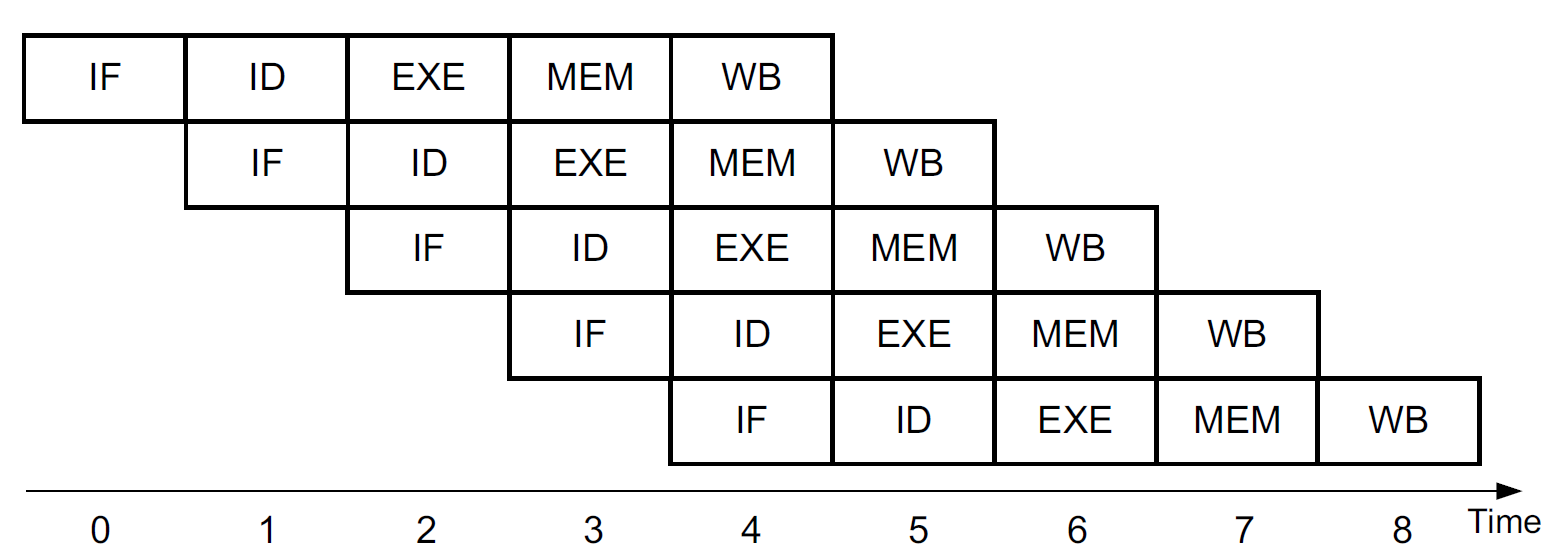
\includegraphics[width=0.8\textwidth]{images/multiProcessor.png}
      \caption{Processor with Multiple Instruction Execution Units}
      \label{multiProcessor}
  \end{center}
\end{figure}

An FPGA does not execute all software on a common computation platform. It executes a
single program at a time on a custom circuit for that program. Therefore, changing the user
application changes the circuit in the FPGA. Given this flexibility, the Vivado HLS compiler does not need to account for overhead stages
in the platform and can find ways of maximizing instruction parallelism. Working with the
same assumptions as in \figref{multiProcessor}, the execution profile of the same software in an FPGA is
shown in \figref{multiFPGA}

\begin{figure}[H]
  \begin{center}
      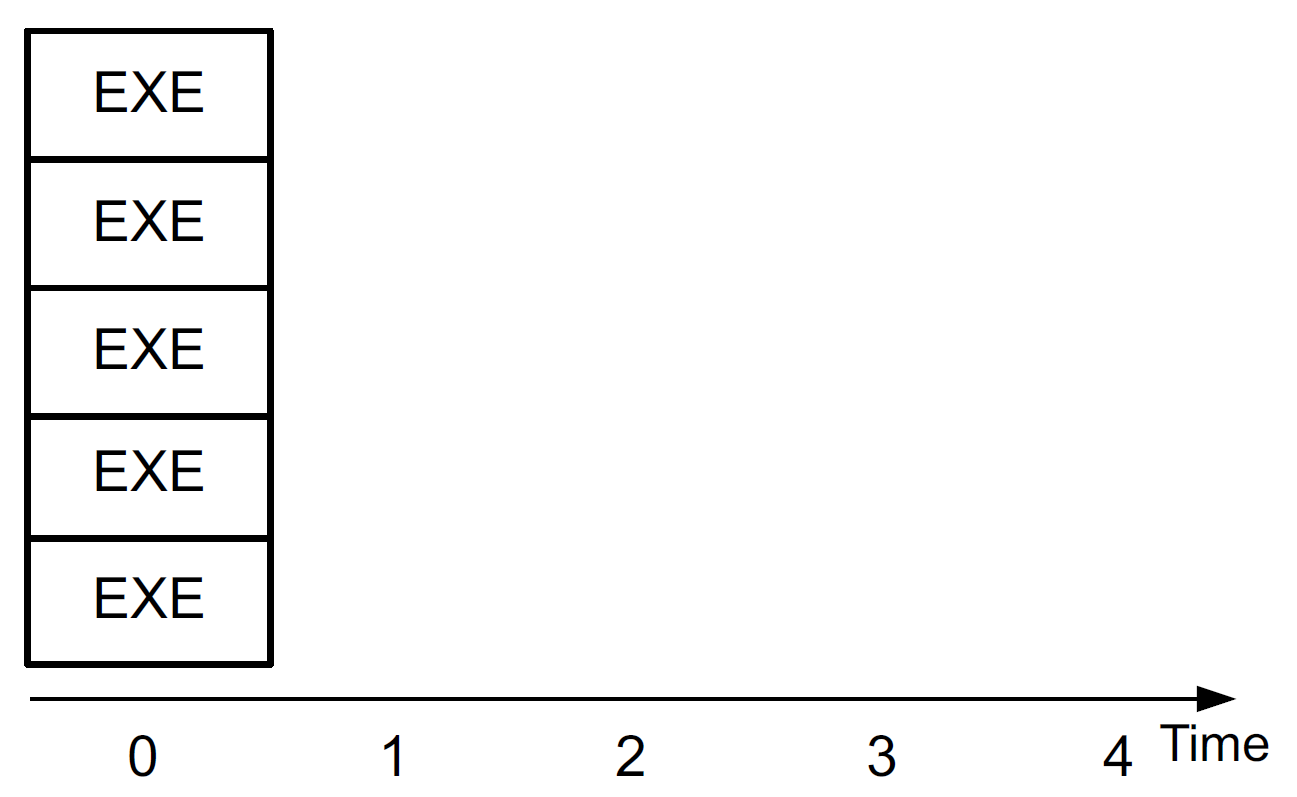
\includegraphics[width=0.6\textwidth]{images/multiFPGA.png}
      \caption{FPGA with Multiple Instruction Execution Units}
      \label{multiFPGA}
  \end{center}
\end{figure}

Based on the comparison of \figref{multiProcessor} and \figref{multiFPGA}, the FPGA has a nominal
performance advantage of 9x compared to the processor. Actual numbers are always
application specific, but FPGAs generally demonstrate at least 10x the performance of a
processor for computationally intensive applications.

\subsubsection{Power Consumption}
Another issue hidden by only focusing on the clock frequency is the power consumption of
a software program. The approximation to power consumption is given by:

\[ P = (1/2) cFV^2 \]

The relationship between power consumption and clock
frequency is supported by empirical data, which shows higher power usage in a processor
than an FPGA for the same computational workload. By creating a custom circuit per
software program, an FPGA is able to run at a lower clock frequency with maximum
parallelism between operations and without the instruction interpretation overhead found
in a processor.

\subsection{Latency and Pipelining}

\textbf{Latency} is the number of clock cycles it takes to complete an instruction or set of instructions to generate an application result value. Using the basic processor architecture, the latency of an instruction is five clock cycles. If the application has
a total of five instructions, the overall latency for this simple model is 25 clock cycles. That is, the result of the application is not available until 25 clock cycles expire. Application latency is a key performance metric in both FPGAs and processors. In both cases, the problem of latency is resolved through the use of pipelining. 

\par In a processor, pipelining means that the next instruction can be launched into execution before the
current instruction is complete. This allows the overlap of overhead stages required in
instruction set processing. By overlapping the execution of instructions, the processor achieves a latency of nine clock cycles for the five instruction application.

\par In an FPGA, the overhead cycles associated with instruction processing are not present. The
latency is measured by how many clock cycles it takes to run the EXE stage of the original
processor instruction. In the case of FPGA, the latency is one clock cycle.Parallelism also plays an important role in latency. For the full five instruction application, the FPGA latency is one clock cycle, as shown in \figref{multiFPGA}. With the one clock cycle latency of
the FPGA, it might not be clear why pipelining is advantageous. However, the reason for
pipelining in an FPGA is the same as in a processor, that is, to improve application
performance.

\par As previously explained, the FPGA is a blank slate with building blocks that must be  connected to implement an application. The Vivado HLS compiler can connect the blocks
directly or through registers. \figref{FPGAWOPipe} shows an implementation of the EXE stages without Pipelining.

\begin{figure}[H]
  \begin{center}
      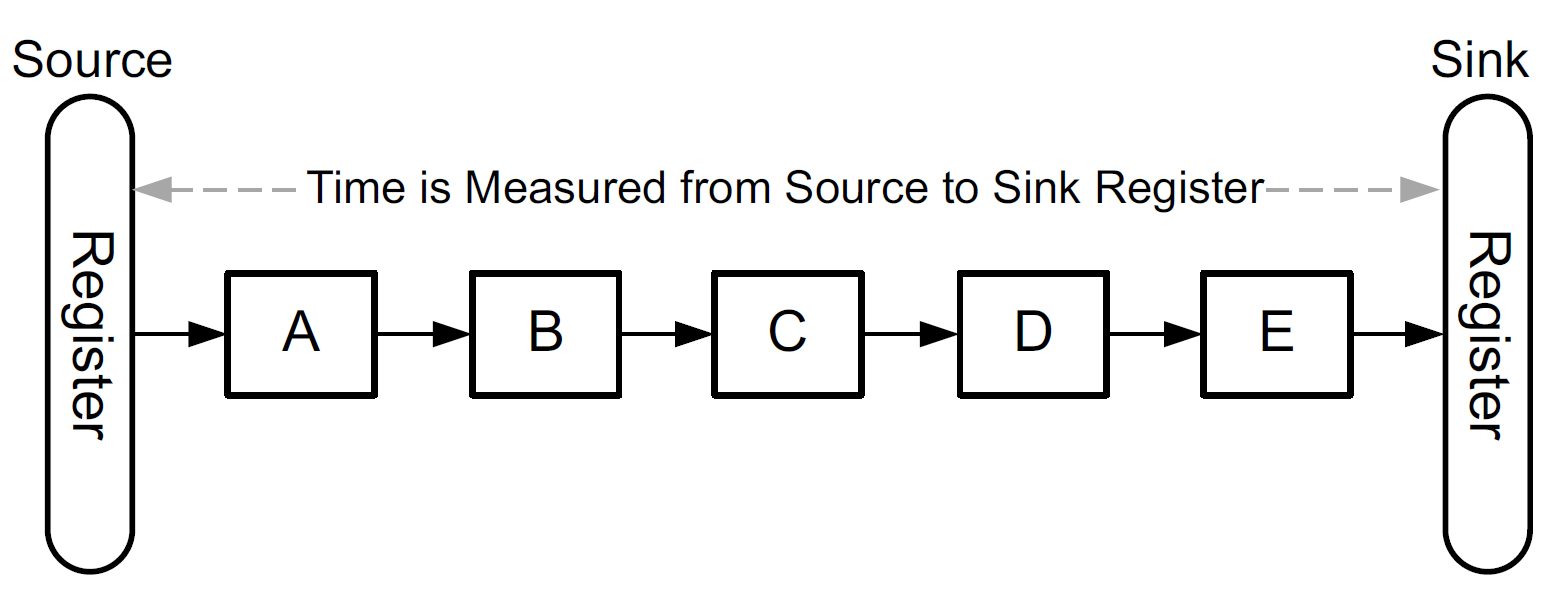
\includegraphics[width=0.6\textwidth]{images/FPGAWOPipe.png}
      \caption{FPGA Implementation without Pipelining}
      \label{FPGAWOPipe}
  \end{center}
\end{figure}

\begin{itemize}
  \item \textbf{Operation timing} in an FPGA is the length of time it takes a signal to travel from a source
  register to a sink register. 
  \item For the case of an FPGA circuit,
  the \textbf{clock frequency} is defined as the longest signal travel time between source and sink
  registers.  
  \item \textbf{Pipelining} in an FPGA is the process of inserting more registers to break up large
  computation blocks into smaller segments. This partitioning of the computation increases
  the latency in absolute number of clock cycles but increases performance by allowing the
  custom circuit to run at a higher clock frequency.
\end{itemize}

\subsubsection{Important points}
\figref{FPGAwithPipe} shows the implementation of the processing architecture in \figref{FPGAWOPipe} after
complete pipelining. Complete pipelining means that a register is inserted between each
building block in the FPGA circuit. 

The addition of registers reduces the timing requirement
of the circuit, which results in a maximum clock frequency. In
addition, by separating the computation into separate register-bounded regions, each
block is allowed to always be busy, which positively impacts the application throughput.

One issue with pipelining is the latency of the circuit. The original circuit of \figref{FPGAWOPipe} has
a latency of one clock cycle at the expense of a low clock frequency. In contrast, the circuit
of \figref{FPGAwithPipe} has a latency of five clock cycles at a higher clock frequency.

\begin{figure}[H]
  \begin{center}
      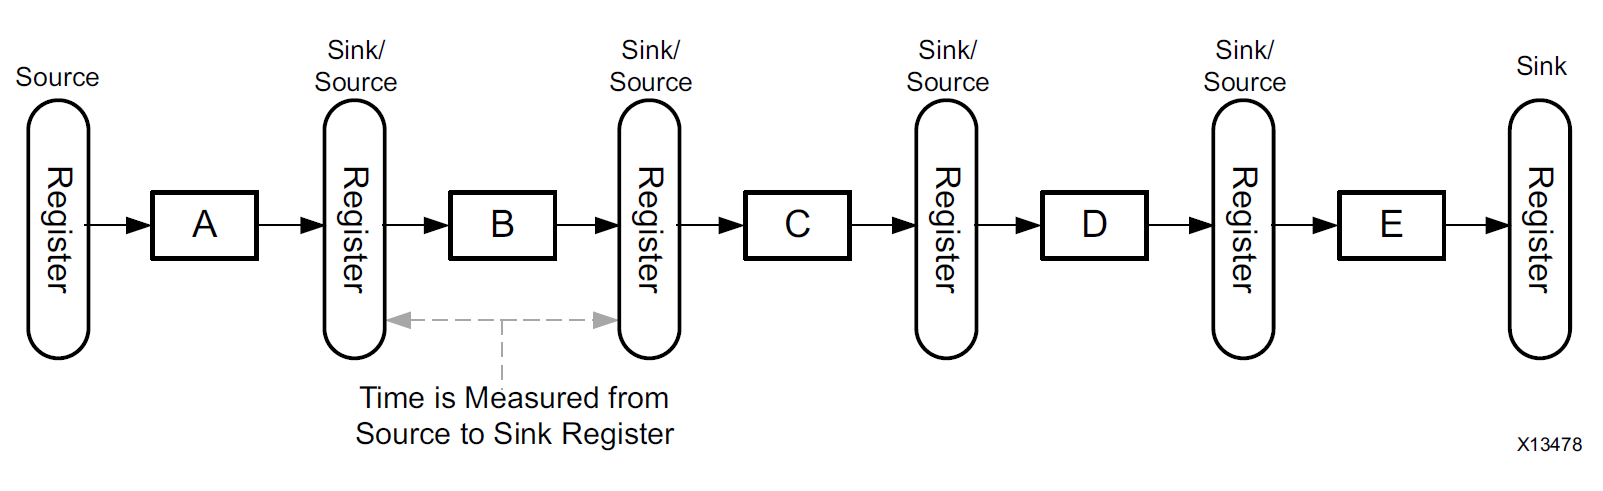
\includegraphics[width=0.8\textwidth]{images/FPGAwithPipe.png}
      \caption{FPGA Implementation with Pipelining}
      \label{FPGAwithPipe}
  \end{center}
\end{figure}

\begin{highlight}
  \textbf{IMPORTANT: The latency caused by pipelining is one of the trade-offs to consider during FPGA design.}
\end{highlight}
\clearpage


\subsection{Throughput}
\textbf{Throughput} is another metric used to determine overall performance of an implementation. It is the number of clock cycles it takes for the processing logic to accept the next input data
sample. With this value, it is important to remember that the clock frequency of the circuit
changes the meaning of the throughput number. 

\par For example, both \figref{FPGAWOPipe} and \figref{FPGAwithPipe} show implementations that require one clock
cycle between input data samples. The key difference is that the implementation in
\figref{FPGAWOPipe} requires 10 ns between input samples, whereas the circuit in \figref{FPGAwithPipe} only
requires 2 ns between input data samples.

\par After the time base is known, it is clear that the
second implementation has higher performance, because it can accept a higher input data
rate.

\begin{highlight}
  Note: The definition of throughput described in this section can also be used when analyzing applications executing on a processor.
\end{highlight}

\subsection{Memory Architecture and Layout}
The memory architecture of the selected implementation platform is one of the physical
elements that can affect the performance of a software application. Memory architecture
determines the upper bound on achievable performance. At some performance point, all
applications on either a processor or an FPGA become memory bound regardless of the
type and number of available computational resources. 


In a processor-based system, the software engineer must fit the application on essentially
the same memory architecture regardless of the specific type of processor. This
commonality simplifies the process of application migration at the expense of performance.
Common memory architecture familiar to software engineers consists of memories that are
slow, medium, or fast based on the number of clock cycles it takes to get the data to the
processor. These memory classifications are defined below.

\begin{table}[H]
  \begin{tabular}{|p{0.15\linewidth} | p{0.80\linewidth}|}
  \hline
  \textbf{Memory Type}    &  \textbf{Definition} \\ \hline
  Slow           & Mass storage devices such as hard drives \\ \hline
  Medium         & DDR memories \\ \hline
  Fast           & On-chip cache memories of different sizes depending on the specific processor \\ \hline
  \end{tabular}
\end{table}

The memory architecture shown in this table assumes that the user is presented with a
single large memory space. Within this memory space, the user allocates and de-allocates
regions to store program data. The physical location of data and how it moves between the
different levels in the hierarchy is handled by the computation platform and is transparent
to the user. In this kind of system, the only way to boost performance is to reuse data in the
cache as much as possible.

\par To achieve this goal, the software engineer must spend large amounts of time looking at
cache traces, restructuring the software algorithm to increase data locality, and managing
memory allocation to minimize the instantaneous memory footprint of the program.

\begin{highlight}
  Although all of these techniques are portable across processors, the results are not. A
  software program must be tuned for each processor it runs on to maximize performance.
\end{highlight}

\par FPGA-based systems can be attached to slow and medium memories
but exhibit the greatest degree of differentiation in terms of available fast memories. That
is, instead of restructuring the software to best use an existing cache, the Vivado HLS
compiler builds a fast memory architecture to best fit the data layout in the algorithm. The
resulting FPGA implementation can have one or more internal banks of different sizes that
can be accessed independently from one another.

\par The use of dynamic memory allocation has long been part of the best practice guidelines for processor-based systems due to the underlying fixed memory architecture.

\par In contrast to this approach, the Vivado HLS compiler builds a memory architecture that is
tailored to the application. This tailored memory architecture is shaped both by the size of
the memory blocks in the program as well as by how the data is used throughout program
execution. Vivado HLS requires that
the memory requirements of an application are fully analyzable at compile time.

\par The benefit of static memory allocation is that Vivado HLS can implement the memory in different ways. Depending on the computation in the algorithm, the Vivado HLS
compiler can implement the memory as registers, shift registers, FIFOs, or BRAMs.

\subsubsection{Registers}
A register implementation of a memory is the fastest possible memory structure. Each independent entity to be stored is embedded into the computation where it is used without the need to address logic or additional delays.

\subsubsection{Shift Register}
In processor programming terms, a shift register can be thought of as a special case of a queue. The key characteristic of a shift register is that every element can be accessed on every clock cycle. In addition, moving all data items to the next adjacent
storage container requires only one clock cycle.

\subsubsection{FIFO}
A FIFO can be thought of as a queue with a single point of entry and a single point of exit. This kind of structure is typically used to transmit data between program loops or functions. There is no addressing logic involved, and the implementation details are completely handled by the Vivado HLS compiler.

\subsubsection{BRAM}
A BRAM is a random-access memory that is embedded into the FPGA fabric. A Xilinx FPGA device includes many of these embedded memories. The exact number of memories is device specific. In processor programming terms, this kind of memory can be thought of as
a cache with the following limitations:

\begin{itemize}
  \item Does not implement cache coherency, collision, and cache miss tracking logic typically found in a processor cache.
  \item Holds its values only as long as the device is powered on (Volatile).
  \item Supports parallel same cycle access to two different memory locations.
\end{itemize}
\clearpage

\section {Vivado High-Level Synthesis}
  The Xilinx Vivado High-Level Synthesis (HLS) compiler provides a programming environment similar to those available for application development on both standard and specialized processors. Vivado HLS shares key technology with processor compilers for the
  interpretation, analysis, and optimization of C/C++ programs. The main difference is in the execution target of the application.
  
  \par By targeting an FPGA as the execution fabric, Vivado HLS enables a software engineer to optimize code for throughout, power, and latency without the need to address the
  performance bottleneck of a single memory space and limited computational resources.
  
  \par Application code targeting the Vivado HLS compiler uses the same categories as any processor compiler. Vivado HLS analyzes all programs in terms of:
  \begin{itemize}
    \item Operations
    \item Conditional statements
    \item Loops
    \item Functions
  \end{itemize}

  
  \begin{highlight}
    IMPORTANT: Vivado HLS can compile almost any C/C++ program. The only coding limitation for Vivado HLS is with dynamic language constructs typical in processors with a single memory space. When using Vivado HLS, the main dynamic constructs to consider are memory allocation and pointers.
  \end{highlight}

                                                    
\subsection{Operations}
Operations refer to both the arithmetic and logical components of an application that are involved in computing a result value. 
\begin{itemize}
  \item With a processor compiler, the fixed processing architecture means that the user can only affect performance by limiting operation dependency and manipulating memory layout to maximize cache performance.
  \item In contrast, Vivado HLS is not constrained by a fixed processing platform and builds an algorithm-specific platform based on user input. This allows an HLS designer to affect application performance in terms of throughput, latency, and power.
\end{itemize} 

\paragraph{Tradeoff between resources, performance, and application}
Although an FPGA does not have a fixed processing architecture, each
device has a maximum number of building blocks it can sustain. Therefore, the designer can evaluate FPGA resources versus application performance versus the number of applications per device.

\subsubsection{Optimizations by vivado HLS}

\begin{itemize}
  \item The scheduling of the operations to reduce the latency is one of the automatic resource optimizations from Vivado HLS.
  \item For memory operations, Vivado HLS analyzes the banks containing the data and where the value is consumed during computation. 
  \item Another way in which Vivado HLS helps the user control the size of the generated circuit is by providing data types for the sizing of variables. Vivado HLS offers the user access to integer, single precision, and double precision data types.
  \item Vivado HLS also offers arbitrary precision data types for eliminating inefficiencies caused due to 32-bit and 64-bit data types.
  \item Arbitrary precision data types reduces the number of resources, the number of levels of logic required to complete an operation, and in the latency of a design.
  \item Based on the size of operations, Vivado HLS automatically does the optimization by pipelining, or division of computation into smaller register-bound regions.
  \item Vivado HLS divides large operators into multiple
  computation stages with a corresponding increase in circuit latency.
\end{itemize}



\subsection{Conditional Statements}
  Conditional statements are program control flow statements that are typically implemented as if, if-else, or case statements. These coding structures are an integral part of most algorithms and are fully supported by all compilers, including HLS. The only difference
  between compilers is how these types of statements are implemented.

  \par With a processor compiler, conditional statements are translated into branch operations that might or might not result in a context switch. The introduction of branches disrupts the maximum instruction execution packing \figref{multiProcessor} by introducing a dependence
  that affects which instruction is fetched next from memory. This uncertainty results in bubbles in the processor execution pipeline and directly affects program performance.

  \par In an FPGA, a conditional statement does not have the same potential impact on  performance as in a processor. Vivado HLS creates all the circuits described by each branch of the conditional statement. Therefore, the runtime execution of a conditional software
  statement involves the selection between two possible results rather than a context switch.


\subsection{Loops}
  Loops are a common programming construct for expressing iterative computation. HLS fully supports loops. The default behavior of HLS is to execute loops in the same schedule as a processor but, HLS can parallelize or pipeline the iterations of a loop to reduce computation latency and increase the input data rate. HLS creates the hardware for the algorithm, it can alter the execution profile of a loop by following optimizations:

  \subsubsection{Optimizations by vivado HLS}
  \begin{enumerate}
    \item To reduce iteration latency, Vivado HLS uses \textbf{Operator Parallelization} to the loop iteration body.
    \item \textbf{Loop Iteration Pipelining} requires user input, as it affects the resource consumption and input data rates of the FPGA implementation.
  \end{enumerate}

  The user controls the level of iteration pipelining by setting the
  \textbf{Loop Initialization Interval (II)}. The II of a loop specifies the number of clock cycles between the start times of consecutive loop iterations. 

  \par To achieve iteration pipelining, HLS analyzes the data dependencies and resource contentions between loop iterations 0 and 1 and automatically resolves issues as follows:
  \begin{itemize}
    \item To resolve data dependencies, HLS alters one of the operations in the loop body or
    queries the user for algorithm changes.
    \item To resolve resource contentions, HLS instantiates more copies of the resource or
    queries the user for algorithm changes.
  \end{itemize}

\subsection{Functions}
  Functions are a programming hierarchy that can contain operators, loops, and other functions. The treatment of functions in both HLS and processor compilers is similar to that
  of loops.

  \par In HLS, the main difference between loops and functions is related to terminology. HLS can parallelize the execution of both loops and functions. To avoid potential confusion when working with HLS, the parallelization
  of function call execution is referred to as \textbf{Dataflow Optimization.}

  The dataflow optimization instructs HLS to create independent hardware modules for all functions at a given level of program hierarchy. These independent hardware modules are capable of concurrent execution and self-synchronize during data transfer.

\subsection{Dynamic Memory Allocation}

Dynamic memory allocation is one of the memory management techniques available in the
C and C++ programming languages. In this method, the user can allocate as much memory
as necessary during program runtime. The size of the allocated memory can vary between
executions of the program and is allocated from a central physical pool of memory. The function calls typically
associated with dynamic memory allocation are shown below:

\begin{table}[H]
  \centering
  \begin{tabular}{|l|l|}
  \hline
  \textbf{C} & \textbf{C++}  \\ \hline
  malloc()   & new()\\ \hline
  calloc()   & delete()\\ \hline
  free()   &  \\ \hline
  \end{tabular}
\end{table} 

As FPGA does not have a fixed memory architecture, HLS synthesizes the memory architecture based on the unique requirements of the
algorithm. Therefore, all code provided to the HLS compiler for implementation in an FPGA
must use compile time analyzable memory allocation only.

\par To aid the user in ensuring that all code provided to HLS is synthesizable, the compiler
executes a coding compliance pass before analyzing the design. This code compliance pass
flags all coding styles that are not suitable for HLS. It is the responsibility of the user to
manually change the code and remove all instances of dynamic memory allocation. 

\begin{highlight}
  Note: HLS cannot synthesize code that includes any of the dynamic memory allocation keywords even if the allocation is constant.
\end{highlight}


\begin{lstlisting}[style=CStyle]
  // Dynamic Memory Allocation in C/C++
  int *A = malloc(10*sizeof(int));
  // This code is not synthesized in HLS.
\end{lstlisting}

There are two possible methods of modifying this code to comply with HLS. 

\paragraph{HLS-Compliant Automatic Memory Allocation}
HLS implements this memory style in strict accordance with the behavior stipulated by C/C++. This means that the memory created to store array A only stores valid data values during the duration of the function call containing this array. Therefore, the function call is
responsible for populating A with valid data before each use.

\paragraph{HLS-Compliant Static Memory Allocation}
The behavior for this type of memory allocation dictates that the contents of array A are valid across
function calls until the program is completely shut down. When working with HLS, the
memory that is implemented for array A contains valid data as long as there is power to the
circuit.

\begin{lstlisting}[style=CStyle]
  // HLS-Compliant Automatic Memory Allocation
  int A[10];

  // HLS-Compliant Static Memory Allocation
  static int A[10];
\end{lstlisting}

Both automatic and static memory allocation techniques can increase the overall software
memory footprint of an algorithm running on a processor.When specifying algorithms in
C/C++ for FPGA implementation, the most important consideration is the overall goal of
the user application. That is, the main goal when compiling to an FPGA is not creating the
best software algorithm implementation. Instead, when using tools like HLS, the goal is to
capture the algorithm in a way that allows the tool to infer the best possible hardware
architecture, which results in the best possible implementation.


\subsection{Pointers}  
A pointer is an address to a location in memory. The HLS compiler supports pointer usage that can be completely
analyzed at compile time. An analyzable pointer usage is usage that can be fully expressed
and computed in a pen and paper computation without the need for runtime information.
  
\begin{lstlisting}[style=CStyle]
  // Valid coding style in which pointers are used to access a
  memory.
  int A[10];
  int *pA;
  pA = A;
\end{lstlisting}      
  

Another supported model for memories and pointers is in accessing external memory.
When using HLS, any pointer access on function parameters implies either a variable or an
external memory. HLS defines an external memory as any memory outside of the scope of
the compiler-generated RTL. This means that the memory might be located in another
function in the FPGA or in part of an off-chip memory, such as DDR.


\clearpage

\section{Software Verification and Vivado HLS}
\subsection{Software Test Bench}
Verification of any HLS-generated module requires a software test bench. The software test
bench serves the following important functions:
\begin{itemize}
    \item To prove that the software targeted for FPGA implementation runs and does not create a segmentation fault.
    \item To prove the functional correctness of the algorithm.
\end{itemize}

\paragraph{Segmentation faults}
Segmentation faults are an issue in HLS as they are in any other compiler. However, there is a difference in how the coding error that caused the issue is detected. 

In a processor-based execution, segmentation faults are caused by a program trying to access a memory location
that is not known to the processor. 
Detection of this error is relatively
straightforward at runtime based on the following sequence of events:
\begin{enumerate}
  \item Processor detects a memory access violation and notifies the operating system (OS).
  \item OS signals the program or process causing the error.
  \item After receiving the error signal from the OS, the program terminates and generates a core dump file for analysis.
\end{enumerate}

\textit{In an HLS-generated implementation, it is difficult to detect a segmentation fault, because
there is no processor and no operating system monitoring program execution.} The only
indicator of a segmentation fault is the appearance of incorrect result values generated by
the circuit. 


\begin{highlight}
  RECOMMENDED: When working with HLS, it is recommended that the designer ensure that the
  software test bench compiles and executes the function without issues on a processor. This guarantees
  that the HLS-generated implementation will not result in a segmentation fault.
\end{highlight}

The other purpose of the software test bench is to prove the functional correctness of an algorithm targeted towards FPGA execution. For the generated hardware implementation,
the HLS compiler guarantees only functional equivalence with the original C/C++ code. Therefore, the existence of a good software test bench is required to minimize efforts in
hardware verification and validation.

A good software test bench is characterized by the execution of thousands or millions of data set tests on the software implementation of an algorithm. This allows the designer to
assert with a high level of confidence that the algorithm was captured properly. However,
even with many test vectors, it is sometimes still possible to detect errors in the
HLS-generated output during hardware verification of an FPGA design. Detecting
functional errors during hardware verification means that the software test bench was
incomplete. Applying the offending test vector to the C/C++ execution reveals the incorrect
statement in the algorithm.

\begin{highlight}
  IMPORTANT: Errors must not be fixed directly in the generated RTL. Any issues with functional
  correctness are a direct result of the functional correctness of the software algorithm.    
\end{highlight}


\begin{highlight}
  TIP: The software test bench used to exercise an algorithm targeted for FPGA implementation with HLS
  does not have any coding style restrictions. The software engineer is free to use any valid C/C++ coding
  style or construct to thoroughly test the functional correctness of an algorithm.    
\end{highlight}


\subsection{Code Coverage}

Code coverage indicates what percentage of the statements in a design are exercised by the
test bench code. This metric, which can be generated by tools like gcov, gives an idea of the
quality of the test vectors used to exercise the algorithm.

\par At a minimum, a test bench must receive a 90\% code coverage score to be considered an adequate test of an algorithm. This means that the test vectors trigger all branches in case statements, conditional if-else statements, and for loops. Aside from the overall coverage
metric, the report generated by code coverage tools provide insight into which parts of a function are executed and which are not.

Running gcov requires that the code is compiled with additional flags that generate the information needed for profiling the execution of a program. Example gcov command on example code named example.c

\begin{lstlisting}[style=CStyle]
  gcc --fprofile-arcs --ftest-coverage example.c
  ./a.out
  gcov example.c    
\end{lstlisting}

\subsection{Uninitialized Variables}
Uninitialized variables are a result of a poor coding style in which the designer does not initialize variables to 0 at the point of declaration. For example, 

\begin{lstlisting}[style=CStyle]
  int A;
  int B;
  ...
  A = B * 100;
\end{lstlisting}

Although some processor compilers resolve the problem by automatically assigning 0 at the point of declaration, HLS does not use this type of solution. HLS assumes that any undefined behavior in the user code can be optimized out of the resulting implementation. This triggers an optimization cascade effect that can reduce the
circuit to nothing. A user can detect this type of error by noticing the empty RTL files for the generated implementation.

\par A better way to detect this type of error is to use code analysis tools, such as \textbf{valgrind \& Coverity}. Both of these tools flag uninitialized variables in the user program. Like all
software quality issues, uninitialized variables must be resolved before the code is compiled with HLS.

\subsection{Out-of-Bounds Memory Access}
In HLS, memory accesses are expressed either as operations on an array or as operations on an external memory through a pointer. In the case of out-of-bounds memory access, the focus is on arrays that are converted into memory blocks by HLS.

\par In a processor compiler, this type of address overflow triggers the address counter to reset to 0.  Although the result is functionally incorrect, this kind of error does not usually result in a program crash.

\par With HLS, accessing an invalid address triggers a series of events that result in an irrecoverable runtime error in the generated circuit. Because the HLS implementation assumes that the software algorithm was properly verified, error recovery logic is not included in the generated FPGA implementation. 

Therefore, an invalid memory address is generated by the implementation of the code to the BRAM resource element. The BRAM then issues an error condition that is not expected by the HLS implementation, and the error is left unattended. The unattended error from the BRAM causes the system to hang and can only be resolved with a device reboot.

\par To catch cases like this before circuit compilation, it is recommended that the tool is executed through a dynamic code checker such as valgrind. Valgrind is a suite of tools designed to check and profile the quality of a C/C++ program. The valgrind Memcheck tool
executes a compiled C/C++ program and monitors all memory operations during execution. This tool flags the following critical issues:
\begin{enumerate}
  \item Use of uninitialized variables
  \item Invalid memory access requests
\end{enumerate}

\begin{highlight}
  RECOMMENDED: Before using HLS to compile a software function for FPGA execution, it is recommended that all of the issues flagged by a dynamic code checker are resolved by the designer.
\end{highlight}



\subsection{Co-Simulation}

Tools for C/C++ program analysis and functionality testing catch most of the issues that affect an HLS implementation. However, these tools are unable to verify whether a sequential C/C++ program maintains functional correctness after parallelization. This issue is resolved in the HLS compiler by the process of co-simulation.

\par Co-simulation is a process in which the generated FPGA implementation is exercised by the
same C/C++ test bench used during software simulation. HLS handles the communication
between the C/C++ test bench and the generated RTL in a manner that is transparent to the
user. As part of this process, HLS invokes a hardware simulator, such as the Vivado simulator,
to emulate how the RTL will function on the device. The main purpose of this simulation is
to check that the parallelization guidance provided by the user did not break the functional
correctness of the algorithm.

\par By default, HLS obeys all algorithm dependencies before parallelization to ensure functional
equivalence with the original C/C++ representation. In cases where an algorithm
dependence cannot be fully analyzed, HLS takes a conservative approach and obeys
dependence. This can lead the compiler to generate a conservative implementation that
does not achieve the target performance goals of the application. 

\par When using co-simulation, it is important to remember that this is a simulation of parallel
hardware being executed on a processor. Therefore, it is approximately 10,000 times slower
than C/C++ simulation. 

\begin{highlight}
  It is also important to remember that the purpose of co-simulation is not to verify the functional correctness of an algorithm. Instead, the purpose is to check that the algorithm was not broken by user guidance to the HLS compiler.
\end{highlight}


\subsection{When C/C++ Verification Is Not Possible}
There are still some cases where the C/C++ representation of an algorithm cannot be fully verified before HLS compilation. 

\par For example, the usage of the
volatile keyword, which is common in device driver development, alerts the compiler
that the pointers are connected to storage elements that might change during the
execution of the function. This kind of pointer must be read or written every time it is
specified in the source code. Traditional compiler optimizations to coalesce pointer
accesses are also turned off by the volatile keyword.

\par The issue with volatile data is that the behavior of the code cannot be fully verified in a
C/C++ simulation. C/C++ simulation does not have the ability to change the value of a
pointer in the middle of the execution of the function under test. Therefore, this type of
code can only be fully verified in an RTL simulation after HLS compilation. The user must
write an RTL test bench to test the generated circuit in all possible cases for each volatile
pointer in the C/C++ source. The use of co-simulation is not applicable in this case, because
it is limited by the test vectors that can be used in a C/C++ simulation.

\clearpage

\section{Design Example: Application Running on a Zynq-7000 SoC}
This design example shows how to take processor code and transform it into an application
that runs on a Zynq-7000 SoC. This example walks through the following steps in the
migration process:

\begin{itemize}
  \item Analyzing and partitioning the processor code
  \item Compiling the program in Vivado HLS
  \item Composing the system in Vivado IP integrator
  \item Connecting processor code and FPGA fabric functions
\end{itemize}

\subsection{Analyzing and partitioning the processor code}
Most software applications targeted for a Zynq-7000 device begin as applications executing on either a standard x86 processor or a DSP processor. Therefore, the first step in migrating a design is to compile the program for the Arm Cortex-A9 processor and analyze its performance. The performance analysis data of a program running on the Arm processor
guides the designer in choosing how to partition the original code between processor and FPGA fabric.

\par Post compilation to the Arm processor, there are two ways of analyzing program performance:
\begin{itemize}
  \item Measuring timing: This method involves instrumenting the code with timers and timing the execution of each sub-function on the processor.
  \item Using code profiling tools: This less intrusive method uses tools, such as gprof, to measure the amount of time spent on a function and to provide statistics on the number of times the function is called.
\end{itemize}

Based on the results of gprof the decision is made where the functions are implemented. After a function is marked for FPGA implementation, the function ports must be analyzed to determine the most suitable hardware interface.


\subsection{Compiling the program in Vivado HLS}

After identifying the functions to run in the FPGA fabric, the designer prepares the source
code for Vivado HLS compilation. 

\begin{highlight}
  RECOMMENDED: When working with multiple projects or modules, it is recommended that the source
  code is separated into different files. This simple technique prevents issues with one module
  compilation affecting the other module in the design.
\end{highlight}

HLS compilation can be controlled using a Tool Command Language (Tcl) script file. A Tcl
script file, which is analogous to a compilation Makefile, instructs the compiler which
function to implement and FPGA device to target. The script is divided into the following sections:

\begin{description}
  \item[Project setup] This section includes the source files and the name of the function to be compiled.
  Guiding the Vivado HLS compiler is an iterative process of applying directives or
  pragmas to the design source code. Each successive refinement of a design is called a
  solution. All projects have at least one solution.
  \item[Solution setup] This section establishes the clock frequency and device for which the software function
  is compiled. If the designer is guiding the compiler through the use of directives, the
  solution directives are included in this section of the script.
  \item[Compilation setup] This section drives the RTL generation and packaging. The assembly of HLS programs
  into an FPGA device application requires the use of the Vivado IP
  integrator, which is a system composition tool. IP integrator requires modules to be
  packed in the equivalent of a software object file.
\end{description}

Interface pragmas define how the module is connected in the FPGA fabric. The definition
process is separated into interface behavior and interface mapping.

\subsection{Composing the system in Vivado IP integrator}
Vivado IP integrator is a Xilinx FPGA design tool for system composition. One use of this
tool is to take the blocks generated by the HLS compiler and connect them into the
processing platform that executes the user application. In software development terms, IP
integrator is analogous to a linker that combines all program objects into a single bitstream.
A bitstream is the binary file used to program the FPGA fabric.

\subsection{Connecting processor code and FPGA fabric functions}
After the FPGA fabric programming binary is created in IP integrator, the designer must
create the software that runs on the processor. The purpose of this software is to initialize
the FPGA fabric functions, launch execution, and receive results from the fabric. For the
overall application to be functionally equivalent to the original processor code, each
function running in the FPGA fabric requires the following functionality in the code running
on the Arm Cortex-A9 processor:

\begin{itemize}
  \item Address mapping
  \item Initialization
  \item Start function
  \item Interrupt service routine (ISR)
  \item Interrupt registration in the processor exception table
  \item New main function to run the system
\end{itemize}

\clearpage

\section{Verification of a Complete Application}

In FPGA design, a complete application refers to a hardware system that implements the
functionality captured by the software representation of a design. There are two main
categories of systems that can be built on an FPGA using the Vivado HLS compiler:
\begin{enumerate}                                      
  \item Standalone Compute Systems                                   
  \item Processor-Based Systems
\end{enumerate}

\subsection{Standalone compute systems}
The standalone compute system is an FPGA implementation created by one or more
HLS-generated modules connected together to implement a software application. In these
types of systems, the configuration of the algorithm is fixed and loaded during device
configuration. The modules generated by the HLS compiler are connected to external FPGA
pins for data transmit and receive transactions. This is the easiest kind of system to verify.
The verification of a standalone system is divided into the following stages:
\begin{enumerate}
  \item Module verification
  \item Connectivity verification
  \item Application verification
  \item Device validation
\end{enumerate}

\subsubsection{Module Verification}
Module verification of an HLS-generated block is covered in section "Software
Verification and Vivado HLS". After the block is fully verified for functional correctness in
both software and co-simulation, the designer must test the block for in system error
tolerance.

\par Both software simulation and co-simulation are focused on testing the functional
correctness of an algorithm in isolation. That is, the algorithm and compiled module are
tested to ensure correct functionality when all inputs and outputs are handled in an ideal
manner. This thorough level of testing helps to ensure correctness after data is supplied to
the module. It also helps to reduce the verification burden of later stages by eliminating the
internal processing core of a module as a possible source of error. \textbf{The only module-level
issue that is not handled by this methodology is verification that the module can recover
fully from incorrect handshaking at its interfaces.}

\par In-system testing tests how the HLS-generated module reacts to incorrect toggling of its
input and output ports. The purpose of this testing is to eliminate I/O behavior as an error
source that can crash or otherwise adversely affect the module under test. The types of
improper use cases tested in this methodology are:

\begin{itemize}
  \item Erratic clock signal toggling
  \item Reset operation and random reset pulsing
  \item Input ports receiving data at different rates
  \item Output ports being sampled at different rates
  \item Interface protocol violations
\end{itemize}

These tests, which are examples of system-level behavior, ensure that the HLS-generated
module functions as expected under all circumstances. The amount of testing required at
this stage depends on the types of interfaces and the integration methodology. By using
HLS default settings to generate AXI-compliant interfaces, the designer can avoid writing
an exhaustive test bench of incorrect system-level behavior. AXI-compliant interfaces are
fully tested and verified by the developers of the HLS compiler.


\subsubsection{Connectivity Verification}
Connectivity verification is a sequence of tests to check that the modules in an application
are properly connected to each other. As with module verification, the amount of testing
required depends on the system integration methodology. FPGA design tool assistance is provided in both the Xilinx System Generator and Vivado IP
integrator design flows. These graphical module connection tools handle all the aspects
related to module connection. 

\par The manual integration flow requires the user to write an application top-level module in
RTL and manually connect the RTL ports of every module that makes up an application. This
is the most error-prone flow and must be verified. The amount of testing required can be
decreased by using HLS compiler defaults and generating AXI interfaces for every module
port.

\par For systems built around AXI interfaces, the connectivity can be verified through the use of
a bus functional model (BFM). The BFM provides the Xilinx-verified behavior of AXI buses
and point-to-point connections. These models can be used for traffic generators, which
help prove the correct connection of HLS-generated modules as part of an RTL simulation.

\begin{highlight}
  IMPORTANT: It is important to remember that the purpose of this simulation is only to check
  connectivity and the proper flow of data through the system. The connectivity verification step does not
  verify the functional correctness of the application.  
\end{highlight}

\subsubsection{Application Verification}
Application verification is the final step before running the application on the FPGA device.
Application verification focuses on checking that the original software model matches the
results of the FPGA implementation. If the application is composed of a single
HLS-generated module, this stage is the same as module verification. In cases where the
application is composed of two or more HLS-generated modules, the verification process
starts with the original software model.
The designer must extract application input and output test vectors from the software
model to be used in an RTL simulation. Because the construction of the hardware
implementation is verified in multiple stages, the application verification does not need to
be an exhaustive simulation. The simulation can run as many test vectors as needed for the
designer to feel confident in the FPGA implementation.

\subsubsection{Device Validation}
After an application is assembled in RTL using either automated or manual integration
flows, the design goes through an additional compilation stage to generate the binary or
bitstream required to program the FPGA. In the terminology of FPGA design, the
compilation of RTL into a bitstream is referred to as logic synthesis, implementation, and
bitstream generation. Once the bitstream is generated, the FPGA device can be
programmed. The application is validated after the hardware runs correctly for an amount
of time specified by the designer.
\clearpage

\subsection{Processor-based systems}
For the module and connectivity verification stages, the verification flow for a
processor-based system is the same as the standalone system. The major difference is that
a portion of the application is running on the processor. 

This partitioning presents a verification
challenge that can be addressed through the use of the following technologies:
\begin{itemize}
  \item Hardware in the loop (HIL) verification
  \item Virtual platform (VP) verification
\end{itemize}

\subsubsection{Hardware in the Loop (HIL) Verification}
HIL verification is a verification methodology in which the simulation of part of the system
under test is executed in the FPGA fabric. The main advantages of HIL verification versus verification are:
\begin{itemize}
  \item No simulation inconsistencies between a processor model and the actual processor
  \item Code running on the processor is executed at the speed of the FPGA device
  \item Full visibility into how each generated module operates through RTL simulation
\end{itemize}

When using HIL verification, it is important to remember the performance characteristics of
this technology. Although the processor code runs in the actual hardware, the FPGA fabric
is fully simulated on the designer’s workstation. HIL verification is
only recommended for verifying the major interactions between the processor and the
FPGA fabric, not every use case in the application. The key application behaviors to check
with HIL verification are:
\begin{itemize}
  \item Vivado HLS driver integration into the processor code
  \item Writing configuration parameters from the PS to the PL
  \item Interrupt from the PL to the PS
\end{itemize}


\subsubsection{Virtual Platform(VP) Verification}
Virtual platform technology is an established method of overlapping software and
hardware development. A virtual platform is a
software simulation of both the application and the hardware platform on which it runs. The
models used for the PL portion of the design can be in C, C++, SystemC, or RTL. This
simulation platform can be used as a proxy for the other recommended verification stages
with varying degrees of fidelity to the hardware implementation.

\par In the fastest use case of the virtual platform, the application modules targeted to the PL
are simulated from the C/C++ source code provided to the Vivado HLS compiler. This setup
results in a functionally correct simulation that allows the designer to test the algorithm for
correct computation. As modules are optimized and compiled with Vivado HLS, the
generated RTL can replace the software version of the module to enable connectivity
testing and timing driver simulation.

\begin{highlight}
  IMPORTANT: It is important to remember that adding RTL modules impacts the runtime on the virtual
  platform and slows down execution.  
\end{highlight}


\subsubsection{Device Validation}
The purpose of device validation is to check all the application use cases in which the
processor interacts with the FPGA fabric. As in the case of standalone execution, this
process involves running the complete application for a certain amount of time on the FPGA/SoC.
The purpose of this test is to check all the application corner cases with
regard to the interaction between the PS and PL portions of the design.


\iffalse

Chapter 5: Computation-Centric Algorithms
  Overview                                                     
  Data Rate Optimization    

Chapter 6: Control-Centric Algorithms
  Overview                                                     
  Expressing Control in C/C++                                  
  UDP Packet Processing    

\fi
  \clearpage

  % \chapter{Vivado High-Level Synthesis}   
  % % \iffalse
% High-Level Synthesis Benefits                   
% High-Level Synthesis Basics                     
% Understanding Vivado HLS                        
% Using Vivado HLS                                
% Data Types for Efficient Hardware               
% Managing Interfaces                             
% Optimizing the Design                           
% Verifying the RTL                               
% Exporting the RTL Design    

% \chapter{High-Level Synthesis C Libraries}
% Arbitrary Precision Data Types Library          
% HLS Stream Library                              
% HLS Math Library                                
% HLS Video Library                               
% HLS IP Libraries                                
% HLS Linear Algebra Library                      
% HLS DSP Library                                 
% HLS SQL Library   

% \chapter{High-Level Synthesis Coding Styles}
% Unsupported C Constructs                        
% C Test Bench                                    
% Functions                                       
% Loops                                           
% Arrays                                          
% Data Types                                      
% C Builtin Functions                             
% Hardware Efficient C Code      

% C++ Classes and Templates                              
% Assertions                                               
% SystemC Synthesis 

% \chapter{High-Level Synthesis Reference Guide}
% Command Reference                                        
% GUI Reference                                            
% Interface Synthesis Reference                            
% AXI4-Lite Slave C Driver Reference                       
% HLS Video Functions Library                              
% HLS Linear Algebra Library Functions                     
% HLS DSP Library Functions                                
% HLS SQL Library Functions                                
% C Arbitrary Precision Types                              
% C++ Arbitrary Precision Types                            
% C++ Arbitrary Precision Fixed-Point Types                
% Comparison of SystemC and Vivado HLS Types               

% \fi

% \section{Introduction}
% The Xilinx Vivado High-Level Synthesis (HLS) tool transforms a C specification into a register transfer level (RTL) implementation that can be synthesized into a Xilinx field programmable gate array (FPGA). C specifications can be written in C, C++, or SystemC, and the FPGA provides a massively parallel architecture with benefits in performance, cost, and power over traditional processors.

% \par Vitis/Vivado HLS is a high-level synthesis tool that allows C, C++, and OpenCL functions to become hardwired onto the device logic fabric and RAM/DSP blocks. Vitis/Vivado HLS implements hardware kernels in the Vitis application acceleration development flow and uses C/C++ code for developing RTL IP for Xilinx device designs in the Vivado Design Suite.

% \section{High-Level Synthesis Benefits}
% High-level synthesis bridges hardware and software domains, providing the following benefits:
% \begin{itemize}
%   \item Improved productivity for hardware designers:\\ Hardware designers can work at a higher level of abstraction while creating high-performance hardware.
%   \item Improved system performance for software designers:\\ Software developers can accelerate the computationally intensive parts of their algorithms on a new compilation target, the FPGA. 
% \end{itemize}

% Using a high-level synthesis design methodology allows you to:
% \begin{itemize}
%   \item Develop algorithms at the C-level:\\ Work at a level that is abstract from the implementation details, which consume development time.
%   \item Verify at the C-level:\\ Validate the functional correctness of the design more quickly than with traditional hardware description languages.
%   \item Control the C synthesis process through optimization directives:\\ Create specific high-performance hardware implementations.
%   \item Create multiple implementations from the C source code using optimization directives:\\ Explore the design space, which increases the likelihood of finding an optimal implementation.
%   \item Create readable and portable C source code:\\ Retarget the C source into different devices as well as incorporate the C source into new projects.
% \end{itemize}

% \section{High-Level Synthesis Basics}   
% High-level synthesis includes the following phases:
% \begin{itemize}
%   \item Scheduling
%     Determines which operations occur during each clock cycle based on:
%     \begin{itemize}
%       \item Length of the clock cycle or clock frequency.
%       \item Time it takes for the operation to complete, as defined by the target device.
%       \item User-specified optimization directives.
%     \end{itemize}
%     If the clock period is longer or a faster FPGA is targeted, more operations are completed within a single clock cycle, and all operations might complete in one clock cycle. Conversely, if the clock period is shorter or a slower FPGA is targeted, high-level synthesis automatically schedules the operations over more clock cycles, and some operations might need to be  implemented as multicycle resources.
%     \item Binding
%     Determines which hardware resource implements each scheduled operation. To implement
%     the optimal solution, high-level synthesis uses information about the target device.
%     \item Control logic extraction
%     Extracts the control logic to create a finite state machine (FSM) that sequences the operations
%     in the RTL design.
% \end{itemize}

% High-level synthesis synthesizes the C code as follows:
% \begin{itemize}
%   \item Top-level function arguments synthesize into RTL I/O ports.
%   \item C functions synthesize into blocks in the RTL hierarchy:\\ If the C code includes a hierarchy of sub-functions, the final RTL design includes a hierarchy of modules or entities that have a one-to-one correspondence with the original C function hierarchy. All instances of a function use the same RTL implementation or block.
%   \item Loops in the C functions are kept rolled by default When loops are rolled, synthesis creates the logic for one iteration of the loop, and the RTL design executes this logic for each iteration of the loop in sequence. Using optimization directives, you can unroll loops, which allows all iterations to occur in parallel. Loops can also be pipelined, either with a finite-state machine fine-grain implementation (loop pipelining) or with a more coarse-grain handshake-based implementation (dataflow).
%   \item Arrays in the C code synthesize into block RAM or UltraRAM in the final FPGA design
%   If the array is on the top-level function interface, high-level synthesis implements the array as
%   ports to access a block RAM outside the design.
%   High-level synthesis creates an optimized implementation based on default behavior, constraints,
%   and any optimization directives you specify. You can use optimization directives to modify and
%   control the default behavior of the internal logic and I/O ports. This allows you to generate
%   variations of the hardware implementation from the same C code.
%   To determine if the design meets your requirements, you can review the performance metrics in
%   the synthesis report generated by high-level synthesis. After analyzing the report, you can use
%   optimization directives to refine the implementation. The synthesis report contains information
%   on the following performance metrics:
%   \item Area: Amount of hardware resources required to implement the design based on the resources
%   available in the FPGA, including look-up tables (LUT), registers, block RAMs, and DSP48s.
%   \item Latency: Number of clock cycles required for the function to compute all output values.
%   \item Initiation interval (II): Number of clock cycles before the function can accept new input data.
%   \item Loop iteration latency: Number of clock cycles it takes to complete one iteration of the loop.
%   \item Loop initiation interval: Number of clock cycles before the next iteration of the loop starts to
%   process data.
%   \item Loop latency: Number of cycles to execute all iterations of the loop.
% \end{itemize}



% HLS includes the following stages:
% \begin{enumerate}
% \item Scheduling determines which operations occur during each clock cycle based on:
%     \begin{itemize}
%         \item When an operation's dependencies have been satisfied or are available.
%         \item The length of the clock cycle or clock frequency.
%         \item The time it takes for the operation to complete, as defined by the target device.
%         \item The available resource allocation.
%         \item Incorporation of any user-specified optimization directives.
%     \end{itemize}
% TIP: More operations can be completed in a single clock cycle for longer clock periods, or if a faster device is targeted, and all operations might complete in one clock cycle. However, for shorter clock periods, or when slower devices are targeted, HLS automatically schedules operations over more clock cycles. Some operations might need to be implemented as multi-cycle resources.
% \item Binding assigns hardware resources to implement each scheduled operation, and maps operators (such as addition, multiplication, and shift) to specific RTL implementations. For example, a mult operation can be implemented in RTL as a combinational or pipelined multiplier.
% \item Control logic extraction creates a finite state machine (FSM) that sequences the operations in the RTL design according to the defined schedule.
% \end{enumerate}

% \subsection{Scheduling}
% Scheduling

% \subsection{Binding}
% Binding assigns hardware resources to implement each 

% \subsection{Control Logic} 
% Control Logic extraction creates a finite state machine (FSM) that sequences the operations in the RTL design according to the defined schedule.


% \section{Understanding Vivado HLS}                        
% \section{Using Vivado HLS}                                
% \section{Data Types for Efficient Hardware}
% \section{Managing Interfaces}                
% \section{Optimizing the Design}                           
% \section{Verifying the RTL}                               
% \section{Exporting the RTL Design}


% Vivado HLS provides a number of optional C libraries to enable higher productivity and high performance RTL design these include arbitrate precision libraries allowing operations to be performed any arbitrary precision for example 10 bit, 25 bit or 42 bits rather than just the standard 8, 16, 32 and 64 bit provided in the C language. Video libraries allowing you to easily implement many of the most popular open CV video functions, unmask linear algebra and DSP libraries providing high quality RTL implementations of sine, cosine, cholesky and Viterbi decoder among others.

% In the Vitis application acceleration flow, the Vitis HLS tool automates much of the code modifications required to implement and optimize the C/C++ code in programmable logic and to achieve low latency and high throughput. The inference of required pragmas to produce the right interface for your function arguments and to pipeline loops and functions within your code is the foundation of Vitis HLS in the application acceleration flow. Vitis HLS also supports customization of your code to implement different interface standards or specific optimizations to achieve your design objectives.

% Following is the Vitis HLS design flow:
% \begin{enumerate}
%     \item Compile, simulate, and debug the C/C++ algorithm.
%     \item View reports to analyze and optimize the design.
%     \item Synthesize the C algorithm into an RTL design.
%     \item Verify the RTL implementation using RTL co-simulation.
%     \item Package the RTL implementation into a compiled object file (.xo) extension, or export to an RTL IP.
% \end{enumerate}
  % \clearpage

  \chapter{Vitis High-Level Synthesis}   
  % UG 1399 document
% Chapter I

\section{Design Principles for Software Programmers}

\subsection{Introduction}
The discussion in this section is tool-agnostic and the concepts introduced are common to most HLS tools. 

\begin{itemize}
  \item \textbf{Throughput} is defined as the number of specific actions executed per unit of time or results produced per unit of time.
  \item \textbf{Performance} is defined as higher throughput with low
  power consumption. Lower power consumption is just as important as higher throughput.
  
\end{itemize}


\subsection{Computer Architecture}

The von Neumann architecture is the basis of almost all computing done today even though it was designed more than 7 decades ago. This architecture was deemed optimal for a large class of
applications and has tended to be very flexible and programmable. 
However, as application demands started to stress the system, CPUs began supporting the execution of multiple
processes. Multithreading and/or Multiprocessing can include multiple system processes (\eg executing two or more programs at the same time), or it can consist of one process that
has multiple threads within it. Multi-threaded programming using a shared memory system
became very popular as it allowed the software developer to design applications by keeping parallelism in mind but with a fixed CPU architecture. 

\par But when multi-threading and the ever-increasing CPU speeds could no longer handle the data processing rates, multiple CPU cores and hyperthreading were used to improve throughput as shown in the figure on the right.

\begin{highlight}
  This general purpose flexibility comes at a cost in terms of power and peak throughput.  
\end{highlight}

To achieve higher throughput, the workload must be closer
to memory, and/or into specialized functional units. So the new challenge is to design a new programmable architecture in such a way that you can maintain just enough programmability while achieving higher performance and lower power costs.

\par A field-programmable gate array (FPGA) provides for this kind of programmability and offers enough memory bandwidth to make this a high-performance and lower power cost solution. Unlike a CPU that executes a program, an FPGA can be configured into a custom hardware circuit that will respond to inputs in the same way that a dedicated piece of hardware would behave.

\par Reconfigurable devices such as FPGAs contain computing elements of extremely flexible granularities, ranging from elementary logic gates to complete arithmetic-logic units such as DSP blocks. At higher granularities, user-specified composable units of logic called kernels can then be strategically placed on the FPGA device to perform various roles. This characteristic of reconfigurable FPGA devices allows the creation of custom macro-architectures and gives FPGAs a big advantage over traditional CPUs/GPUs in utilizing application-specific parallelism. Computation can be spatially mapped to the device, enabling much higher operational throughput than processor-centric platforms. Today's latest FPGA devices can also contain processor cores (Arm-based) and other hardened IP blocks that can be used without having to program them into the programmable fabric.

\subsection{Three Paradigms for Programming FPGAs}

While FPGAs can be programmed using lower-level Hardware Description Languages (HDLs) such as Verilog or VHDL, there are now several High-Level Synthesis (HLS) tools that can take an algorithmic description written in a higher-level language like C/C++ and convert it into lower-level hardware description languages such as Verilog or VHDL. This can then be processed by downstream tools to program the FPGA device. The main benefit of this type of flow is that you
can retain the advantages of the programming language like C/C++ to write efficient code that can then be translated into hardware. 

\par A program written in C/C++ is essentially written for the von Neumann style of architecture where each instruction is executed sequentially. In order to achieve high performance, the HLS tool must infer parallelism in the sequential code and exploit it to achieve
greater performance. 

\par Many coding techniques (such as RTTI, recursion,
and dynamic memory allocation) have no direct equivalency in hardware. Hence, arbitrary, off-the-shelf software cannot be efficiently converted into hardware. At a bare minimum, such software needs
to be examined for non-synthesizable constructs and the code needs to be refactored to make it synthesizable. Even the automatically converted (or synthesized) program with acceptable quality of results (QoR), will require additional work to help the HLS tool achieve the desired performance goals. 

\subsubsection{Producer-Consumer Paradigm}
In a multithreaded program, there is usually a master
thread that performs some initialization steps and then forks off a number of child threads to do some parallel computation and when all the parallel computation is done, the main thread
collates the results and writes to the output. 

\par Similarly, in FPGAs, same fork/join type of parallelism is applied.
A key pattern for throughput on FPGAs is the producer-consumer paradigm. The producerconsumer
paradigm is applied to a sequential program and it is converted to extract functionality that can be executed in parallel to improve performance. The goal is to decompose the program in such a way
that you can identify tasks that can potentially execute in parallel and therefore increase the throughput of the system.

\par The first step is to understand the program workflow and identify the independent tasks or functions. Two independent tasks need not wait to happen sequentially instead, they can start the execution with interleaving/overlapping. This is referred as Producer-Consumer Paradigm. On FPGAs, due to the custom architecture, the producer and consumer threads can be executed simultaneously with little or no overhead leading to a considerable improvement in throughput unlike a regular CPU. 

\subsubsection{Streaming Data Paradigm "Dataflow"}
A stream is an important abstraction: it represents an unbounded, continuously updating data set, where unbounded means "of unknown or of unlimited size". A stream can be a sequence of data
(scalars or buffers) flowing unidirectionally between a source (producer) process and a destination (consumer) process. 

\par Decomposing your algorithm into producerconsumer
relationships that communicate by streaming data through the network has several advantages. 

\begin{itemize}
  \item It lets the programmer define the algorithm in a sequential manner and the parallelism is extracted through other means (such as by the compiler). 
  \item Complexities like synchronization between the tasks etc. are abstracted away.
  \item It allows the producer and the consumer tasks to process data simultaneously, which is key for achieving higher throughput.
  \item Another benefit is cleaner and simpler code.
\end{itemize}


\subsubsection{Pipelining Paradigm}
Another optimization that allows for finer-grained parallelism is pipelining. Pipelining is a process which enables parallel execution of program instructions. 

\begin{highlight}
  Pipelining does not decrease the latency, that is, the total time for one item to go through the whole system. It does however increase the system's throughput, that is, the rate at which new
  items are processed after the first one.
\end{highlight}

\begin{itemize}
  \item Delay associated with the number of clock cycles lost before the first valid output is delivered is referred to as \textit{Iteration Latency}.
  \item \textit{Initiation Interval (II)} of the pipeline is defined as the time taken by the design between delivering two consecutive outputs post Iteration Latency or first output.  
  \item The overall time taken to deliver all the outputs through iterations is referred to as the \textit{Total Latency} of the pipeline.
\end{itemize}

\begin{highlight}
  Total Latency = Iteration Latency + II * (iterations - 1)  
\end{highlight}

Pipelining is a classical micro-level architectural optimization that can be applied to multiple levels of abstraction. Similar tp task-level pipelining with the producer-consumer paradigm, pipelining applies to the instruction-level as well. This is in fact key to keeping the producer-consumer pipelines (and streams) filled and busy. The producer-consumer pipeline will only be efficient if each task produces/consumes data at a high rate, and hence the need for the
instruction-level pipelining (ILP).

\subsection{Combining the Three Paradigms}
Functions and loops are the main focus of most optimizations in the user's program. Each function can be
converted into a specific hardware component. Each such hardware component can be instantiated in
the hardware design. Each hardware component will in turn be composed of many
smaller predefined components that typically implement basic functions such as add, sub, and
multiply etc. Functions may call other functions although recursion is not supported. 

\par Functions that
are small and called less often can be also inlined into their callers just like how software
functions can be inlined. In this case, the resources needed to implement the function are
subsumed into the caller function's component which can potentially allow for better sharing of
common resources. Constructing your design as a set of communicating functions lends to inferring parallelism when executing these functions.

\begin{highlight}
  An inline function is a function for which the compiler copies the code from the function definition directly into the code of the calling function rather than creating a separate set of instructions in memory. This eliminates call-linkage overhead and can expose significant optimization opportunities.   
\end{highlight}

Loops are one of the most important constructs in your program. Since the body of a loop is
iterated over a number of times, this property can be easily exploited to achieve better
parallelism. There are several transformations (such as {\it pipelining} and {\it unrolling}) that can be made
to loops and loop nests in order to achieve efficient parallel execution. These transformations
enable both memory-system optimizations as well as mapping to multi-core and SIMD execution
resources.

\par In multiple cases, programs are expressed as operations
over large data structures with data dependencies across the
iterations of the loop. Such data dependencies impact the parallelism achievable in the loop. In many such cases, the code must be restructured such that loop iterations can be executed
efficiently and in parallel on modern parallel platforms.

\par An efficient technique to improve throughput and reuse computational resources is to pipeline operators, loops, and/or functions.

\begin{highlight}
  The three paradigms show how parallelism can be
  achieved in the design without needing the complexities of multi-threading and/or parallel programming languages. 
\end{highlight} 

\subsection{Conclusion - A Prescription for performance}
Checklist of high-level actions for achieving performance on reconfigurable FPGA platforms:

\begin{itemize}
  \item Software written for CPUs and software written for FPGAs is fundamentally different. 
  \item Right from the start of your project, establish a flow that can functionally verify the source code changes that are being made. Testing the software against a reference model or using golden vectors are common practices.
  \item (\textbf{Producer - Consumer Paradigm: })Focus first on the macro-architecture of your design.
  \item Visualize parallelism with function execution timeline and compare with the final achieved results.
  \item Only start coding or refactoring your program once you have the macro-architecture and the activity timeline established.
  \item As a general rule, the HLS compiler will only infer task-level parallelism from function calls.
  \item \textbf{Data flow: } Decompose/partition the original algorithm into smaller components that talk to each other via streams (Visualize the data flow).
  \begin{itemize}
    \item Smaller modular components have the advantage that they can be replicated when needed to improve parallelism.
    \item Avoid having communication channels with very wide bit-widths. Decomposing such wide channels into several smaller ones will help implementation on FPGA devices.
    \item Large functions (written by hand or generated by inlining smaller functions) can have nontrivial control paths that can be hard for tools to process.
    \item Smaller functions with simpler control paths will aid implementation on FPGA devices.
    \item Aim to have a single loop nest (with either fixed loop bounds that can be inferred by HLS tool, or by providing loop trip count information by hand to the HLS tool) within each function. This greatly facilitates the measurement and optimization of throughput. (Not be applicable for all designs)
    \item 
  \end{itemize}
  \item \textbf{Throughput: } Have an overall vision about what rates of processing will be required during each phase of your design is important. Knowing this will influence how you write your application for FPGAs.
  \begin{itemize}
    \item Try to locate the critical path(s) in the design a potential bottleneck.  
    \item HLS GUI tools and/or the simulation waveform viewer can be used to visualize such throughput issues.
    \item Stream-based communication allows consumers to start processing as soon as producers start producing which allows for overlapped execution (which in turn increases parallelism
    and throughput).
    \item In order to keep the producer and consumer tasks running constantly without any hiccups, optimize the execution of each task to run as fast as possible using techniques such as
    pipelining and the appropriate sizing of streams.    
  \end{itemize}
  \item Think about the granularity (and overhead) of the streaming channels with respect to synchronization. 
  \item PIPO and FIFO : The usage of PIPO channels allows you to overlap task execution without the fear of deadlock while explicit manual streaming FIFO channels allow you to start the overlapped execution sooner (than PIPOs) but require careful adjustment of FIFO sizes to avoid deadlocks.
  \item Locate and remove un-synthesizable C/C++ coding styles.
  \item Use the reports generated by the HLS compiler to guide the optimization process. 
  \item Another important aspect to consider is the interface of accelerated function or kernel. The interface of the kernel to the outside world is an important element of the eventual system design.
\end{itemize}



\clearpage
\section{Introduction to Vitis/Vivado HLS}

Vitis/Vivado HLS is a high-level synthesis tool that allows C, C++, and OpenCL functions to become hardwired onto the device logic fabric and RAM/DSP blocks. Vitis/Vivado HLS implements hardware kernels in the Vitis application acceleration development flow and uses C/C++ code for developing RTL IP for Xilinx device designs in the Vivado Design Suite.

\par In the Vitis application acceleration flow, the Vitis/Vivado HLS tool automates much of the code modifications required to implement and optimize the C/C++ code in programmable logic and to achieve low latency and high throughput. The inference of required pragmas to produce the right interface for your function arguments and to pipeline loops and functions within your code is the foundation of Vitis/Vivado HLS in the application acceleration flow. Vitis/Vivado HLS also supports customization of your code to implement different interface standards or specific optimizations to achieve your design objectives.

Following is the Vitis/Vivado HLS design flow:
\begin{enumerate}
    \item Compile, simulate, and debug the C/C++ algorithm.
    \item View reports to analyze and optimize the design.
    \item Synthesize the C algorithm into an RTL design.
    \item Verify the RTL implementation using RTL co-simulation.
    \item Package the RTL implementation into a compiled object file (.xo) extension, or export to an RTL IP.
\end{enumerate}

\subsection{High-Level Synthesis Benefits}
High-level synthesis bridges hardware and software domains, providing the following benefits:
\begin{itemize}
  \item Improved productivity for hardware designers:\\ Hardware designers can work at a higher level of abstraction while creating high-performance hardware.
  \item Improved system performance for software designers:\\ Software developers can accelerate the computationally intensive parts of their algorithms on a new compilation target, the FPGA. 
\end{itemize}

Using a high-level synthesis design methodology allows you to:
\begin{description}
  \item[Develop algorithms at the C-level] Work at a level that is abstract from the implementation details, which consume development time.
  \item[Verify at the C-level] Validate the functional correctness of the design more quickly than with traditional hardware description languages.
  \item[Control the C synthesis process through optimization directives] Create specific high-performance hardware implementations.
  \item[Create multiple implementations from the C source code using optimization directives] Explore the design space, which increases the likelihood of finding an optimal implementation.
  \item[Create readable and portable C source code] Retarget the C source into different devices as well as incorporate the C source into new projects.
\end{description}

\subsection{High-Level Synthesis Basics}   
High-level synthesis includes the following phases:
\begin{itemize}
  \item Scheduling
    Determines which operations occur during each clock cycle based on:
    \begin{itemize}
      \item Length of the clock cycle or clock frequency.
      \item Time it takes for the operation to complete, as defined by the target device.
      \item User-specified optimization directives.
      \item Operation's dependencies.
      \item Available resource allocation.
    \end{itemize}
    If the clock period is longer or a faster FPGA is targeted, more operations are completed within a single clock cycle, and all operations might complete in one clock cycle. Conversely, if the clock period is shorter or a slower FPGA is targeted, high-level synthesis automatically schedules the operations over more clock cycles, and some operations might need to be  implemented as multicycle resources.
    \item Binding
    Determines which hardware resource implements each scheduled operation. To implement
    the optimal solution, high-level synthesis uses information about the target device.
    \item Control logic extraction
    Extracts the control logic to create a finite state machine (FSM) that sequences the operations
    in the RTL design.
\end{itemize}

\clearpage
\section{Vitis/Vivado HLS Process Overview}
Vitis/Vivado HLS is project based and can contain multiple variations called "solutions" to drive synthesis
and simulation. Each solution can target either the Vivado IP flow, or the Vitis Kernel flow. Based
on the target flow, each solution will specify different constraints and optimization directives.

\par The following are the synthesis, analysis, and optimization steps in the typical design flow:
\begin{enumerate}
  \item Create a new Vitis/Vivado HLS project.
  \item Verify the source code with C simulation.
  \item Run high-level synthesis to generate RTL files.
  \item Analyze the results by examining latency, initiation interval (II), throughput, and resource utilization.
  \item Optimize and repeat as needed.
  \item Verify the results using C/RTL Co-simulation.
\end{enumerate}

Vitis/Vivado HLS implements the solution based on the target flow, default tool configuration, design
constraints, and any optimization pragmas or directives you specify. You can use optimization
directives to modify and control the implementation of the internal logic and I/O ports,
overriding the default behaviors of the tool.

\par The C/C++ code is synthesized as follows:
\begin{itemize}
  \item Top-level function arguments synthesize into RTL I/O port interfaces automatically by Vitis/Vivado HLS. 
  \item Sub-functions of the top-level C/C++ function synthesize into blocks in the hierarchy of the RTL design.
  \begin{itemize}
    \item The final RTL design includes a hierarchy of modules or entities that correspond with the original top-level C function hierarchy.
    \item Vitis/Vivado HLS automatically inlines sub-functions into higher level functions, or the top-level function as needed to improve performance.
    \item By default, each call of the C sub-function uses the same instance of the RTL module.
  \end{itemize}
  \item Loops in the C functions are kept rolled and are pipelined by default to improve performance.
  \begin{itemize}
    \item The Vitis/Vivado HLS tool will not unroll loops unless it improves the performance of the solution. 
    \item Loops can be manually unrolled.
    \item Loops can also be pipelined, either with a finite-state machine fine-grain implementation (loop pipelining) or with a more coarse-grain handshake-based implementation (dataflow).
  \end{itemize}
  \item Arrays in the code are synthesized into block RAM (BRAM), LUT RAM, or UltraRAM in the final FPGA design.
  \begin{itemize}
      \item If the array is on the top-level function interface, high-level synthesis implements the array as ports with access to a block RAM outside the design.
      \item The type of memory used can be reconfigured, or read/write memory transfers can be reconfigured.
  \end{itemize}
\end{itemize}

After synthesis, you can analyze the results in the various reports produced to determine the quality of your results. After analyzing the results, you can create additional solutions for your
project specifying different constraints and optimization directives, and synthesize and analyze
those results. You can compare results between different solutions to see what has worked and
what has not. You can repeat this process until the design has the desired performance
characteristics. Using multiple solutions allows you to proceed with development while retaining
prior solutions.


\par These are the performance metrics:
\begin{itemize}
  \item Area: Amount of hardware resources required to implement the design based on the resources
  available in the FPGA, including look-up tables (LUT), registers, block RAMs, and DSP48s.
  \item Latency: Number of clock cycles required for the function to compute all output values.
  \item Initiation interval (II): Number of clock cycles before the function can accept new input data.
  \item Loop iteration latency: Number of clock cycles it takes to complete one iteration of the loop.
  \item Loop initiation interval: Number of clock cycles before the next iteration of the loop starts to
  process data.
  \item Loop latency: Number of cycles to execute all iterations of the loop.
\end{itemize}

\clearpage
\section{Creating project with Vitis HLS}
Inputs of the Vitis/Vivado HLS are:
\begin{itemize}
  \item \textbf{C function written in C, C++11, C++14, or SystemC}\\ is the primary input to Vitis/Vivado HLS. The function can contain a hierarchy of subfunctions.
  \item \textbf{Constraints}\\ are required and include the clock period, clock uncertainty, and FPGA target. The clock uncertainty defaults to 12.5\% of the clock period if not specified.
  \item \textbf{Directives}\\ are optional and direct the synthesis process to implement a specific behavior or optimization.
  \item \textbf{C test bench and any associated files}\\ are needed to simulate the C function prior to synthesis and to verify the RTL output using C/RTL Cosimulation.
\end{itemize}

Outputs of the Vitis/Vivado HLS are:
\begin{itemize}
  \item \textbf{RTL implementation files in hardware description language (HDL) formats}\\ This is the primary output from Vitis/Vivado HLS. RTL IP produced by Vitis/Vivado HLS is available in both Verilog (IEEE 1364-2001), and VHDL (IEEE 1076-2000) standards, and can be synthesized and implemented into Xilinx devices.
  \item \textbf{Report files}\\ This output is the result of synthesis, C/RTL co-simulation, and IP packaging.
  \item \textbf{Compiled object files (.xo)(Vitis)}\\ This output lets you create compiled hardware functions for use in the Vitis application acceleration development flow. Vitis/Vivado HLS produces this output when called as part of the compilation process from the Vitis tool flow, or when invoked as a stand-alone tool in the bottom up flow.
\end{itemize}

The \figref{VitisFlow} shows an overview of the Vitis/Vivado HLS input and output files.
\begin{figure}[H]
  \begin{center}
      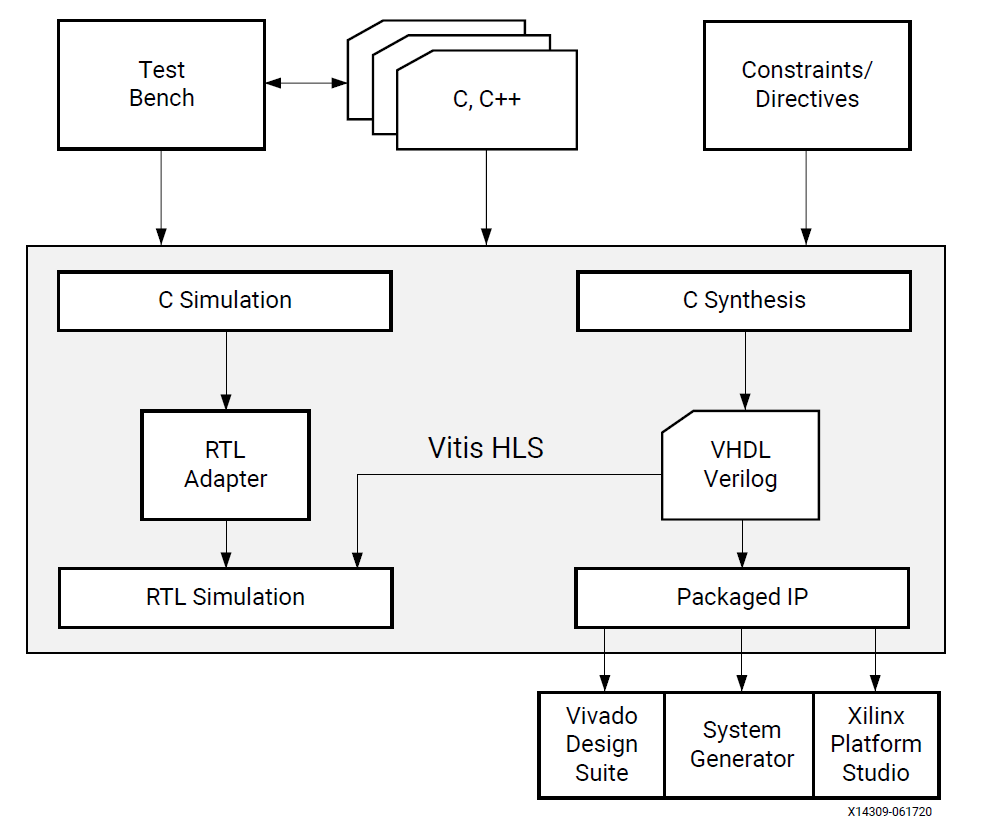
\includegraphics[width=0.7\textwidth]{images/VitisFlow.png}
      \caption{Vitis/Vivado HLS Design Flow}
      \label{VitisFlow}
  \end{center}
\end{figure}

\subsection{Coding C/C++ Functions}
\subsubsection{Coding Style}
In any C program, the top-level function is called main(). In the Vitis HLS design flow, you can specify any sub-function below main() as the top-level function for synthesis. You cannot
synthesize the top-level function main(). Following are additional rules:
\begin{itemize}
  \item Only one function is allowed as the top-level function for synthesis.
  \item Any sub-functions in the hierarchy under the top-level function for synthesis are also synthesized.
  \item If you want to synthesize functions that are not in the hierarchy under the top-level function for synthesis, you must merge the functions into a single top-level function for synthesis.
\end{itemize}

\subsubsection{C/C++ Language Support}
Vitis HLS supports the C/C++ 11/14 for compilation/simulation. 
Vivado HLS supports the following standards for C compilation/simulation: ANSI-C (GCC 4.6), C++ (G++ 4.6), SystemC (IEEE 1666-2006, version 2.2).

Vitis/Vivado HLS supports many C and C++ language constructs, and all native data types for each language, including float and double types. However, synthesis is not supported for some constructs, including:
\begin{itemize}
  \item \textbf{Dynamic memory allocation}\\  An FPGA has a fixed set of resources, and the dynamic creation and freeing of memory resources is not supported.
  \item \textbf{Operating system (OS) operations}\\  All data to and from the FPGA must be read from the input ports or written to output ports. OS operations, such as file read/write or OS queries like time and date, are not supported. Instead, the host application or test bench can perform these operations and pass the data into the function as function arguments.
\end{itemize}

\subsubsection{Libraries in Vitis HLS}
Vitis HLS provides foundational C libraries allowing common hardware design constructs and functions to be easily modeled in C and synthesized to RTL. Vitis HLS provides the following C libraries to extend the standard C languages:

\begin{itemize}
  \item Arbitrary Precision Data Types Library: Arbitrary precision data types let your C code use variables with smaller bit-widths than standard C or C++ data types, to enable improved performance and reduced area in hardware.
  \item Vitis HLS Math Library: Used to specify standard math operations for synthesis into RTL and implementation on Xilinx devices.
  \item HLS Stream Library: For modeling and compiling streaming data structures.
  \item In addition, the Vitis accelerated libraries are available for use with Vitis HLS, including common functions of math, statistics, linear algebra and DSP; and also supporting domain specific applications, like vision and image processing, quantitative finance, database, data analytics, and data compression. Documentation for the Vitis accelerated libraries can be found at \url{https://xilinx.github.io/Vitis_Libraries/}
\end{itemize}

\subsection{Specifying the Clock Frequency}
For C and C++ designs only a single clock is supported. The same clock is applied to all functions in the design. The clock period, can be set in a particular solution. Vitis HLS uses the concept of a clock uncertainty to provide a user defined timing margin. The default clock uncertainty, when it is not specified, is 27\% of the clock period.

\par Using the clock frequency and device target information Vitis HLS estimates the timing of operations in the design but it cannot know the final component placement and net routing:
these operations are performed by logic synthesis of the output RTL. As such, Vitis HLS cannot estimate the exact delays.

\par Vitis HLS aims to satisfy all constraints: timing, throughput, latency. However, if a constraints cannot be satisfied, Vitis HLS always outputs an RTL design.

\clearpage
\section{C simulation verification}
Verification in the Vitis HLS flow can be separated into two distinct processes.
\begin{enumerate}
  \item Pre-synthesis validation that the C program correctly implements the required functionality which is referred to as \textbf{C simulation}.
  \item Post-synthesis verification that the generated RTL code performs as expected which is referred to as \textbf{C/RTL co-simulation}.
\end{enumerate}

Using C to develop and validate the algorithm before synthesis is much faster than developing and debugging RTL code. Vitis HLS uses the test bench to compile and execute the C simulation. Vitis HLS also uses the same test bench to verify the RTL output of synthesis during C/RTL Co-Simulation in Vitis HLS. The first step in high-level synthesis should be to validate the C code functionality, before generating RTL code, by performing simulation using a well written test bench.
  
\subsection{Writing a Test Bench}
\begin{enumerate}
  \item A C test bench includes a main() as a top-level function, that calls the function to be synthesized by the Vitis HLS project.
  \item The test bench includes the main() function which verifies the top-level functionality for synthesis by providing stimuli and calling the function for synthesis, and by consuming and validating its output.
  \item The test bench should execute the top-level function for multiple transactions, allowing many different data values to be applied and verified. 
  \item The test bench is only as good as the variety of tests it performs. 
  \item In addition, the test bench must provide multiple transactions if II is to be calculated during RTL simulation.
  \item The test bench should ideally be \textbf{Self-checking}, and should validate the results from the function to be synthesized are correct.
  \item If the results are correct the test bench returns a value of 0 to main(). Otherwise, the test bench should return any non-zero value.
  \item The test bench can return any non-zero value. A complex test bench can return different values depending on the type of failure. If the test bench returns a non-zero value after C simulation or  C/RTL co-simulation, Vitis HLS reports an error and simulation fails.
  \item As Vitis HLS reuses the C test bench for RTL verification, it requires that the test bench and any associated files be denoted as test bench files when they are added to the Vitis HLS project.
\end{enumerate}


\clearpage
\section{C Synthesis}
During C synthesis, the C/C++ source code is synthesized into an RTL implementation.

Parameters of the C synthesis:
\begin{itemize}
  \item Latency: Number of clock cycles required for the function to compute all output values.
  \item Initiation interval (II): Number of clock cycles before the function can accept new input data.
  \item Loop iteration latency: Number of clock cycles it takes to complete one iteration of the loop.
  \item Loop iteration interval: Number of clock cycles before the next iteration of the loop starts to
  process data.
  \item Loop latency: Number of cycles to execute all iterations of the loop.
  \item Resource Utilization: Amount of hardware resources required to implement the design based on the resources available in the FPGA, including look-up tables (LUT), registers, block RAMs, and DSP blocks.
\end{itemize}

\clearpage
\section{Analyzing the Results of Synthesis}
After synthesis completes, Vitis HLS automatically creates synthesis reports to help you understand and analyze the performance of the implementation. Examples of these reports include the Synthesis Summary report, Schedule Viewer, Function Call Graph, and Dataflow Viewer.

\begin{itemize}
  \item \textbf{Schedule Viewer}: Shows each operation and control step of the function, and the clock cycle that it executes in.
  \item \textbf{Dataflow Viewer}: Shows the dataflow structure inferred by the tool, inspect the channels (FIFO/PIPO), to let you examine the effect of channel depth on performance.
  \item \textbf{Function Call Graph Viewer}: Displays your full design after C Synthesis or C/RTL Cosimulation to show the throughput of the design in terms of latency and II.
\end{itemize}

The Vitis HLS tool also provides additional views to expand on the information available for analysis of your design.

\begin{itemize}
  \item \textbf{Module Hierarchy}: Shows the resources and latency contribution for each block in the RTL hierarchy It also indicates any II or timing violations. In case of timing violations, the hierarchy
  window will also show the total negative slack observed in a specific module.
  \item \textbf{Performance Profile}: Shows details on the performance of the block currently selected in the Module Hierarchy view. Performance is measured in terms of latency and the initiation interval, and includes details on whether the block was pipelined or not.
  \item \textbf{Resource Profile}: Shows the resources used at the selected level of hierarchy, and shows the control state of the operations used.
  \item \textbf{Properties view}: Shows the properties of the currently selected control step or operation in the Schedule Viewer. 
\end{itemize}

\subsection{Schedule Viewer}
The Schedule Viewer provides a detailed view of the synthesized RTL, showing each operation and control step of the function, and the clock cycle that it executes in. It helps you to identify any loop dependencies that are preventing parallelism, timing violations, and data dependencies. The Schedule Viewer is displayed by default in the Analysis perspective.

\subsection{Function Call Graph Viewer}
The new Function Call Graph Viewer, which can be opened from the Flow Navigator, illustrates your full design after C Synthesis or C/RTL Co-simulation. The goal of this viewer is to show the throughput of the design in terms of latency and II. It helps identify the critical path in your design and helps you identify bottlenecks in the design to focus on to improve throughput. It can also show the paths through the design where throughput may be imbalanced leading to FIFO stalls and/or deadlock.

\par In some cases, the displayed hierarchy of the design might not be the same as your source code
as a result of HLS optimizations that convert loops into function pipelines, etc. Functions that are
in-lined will no longer be visible in the call graph, as they are no longer separate functions in the
synthesized code. If multiple instances of a function are created, each unique instance of the function is shown in the call graph. 

\par The call graph displays functions as rectangular boxes, and loops as oval boxes, each with II, latency, and resource or timing data depending on the specific view. Before C/RTL cosimulation is completed the performance and resource metrics that are shown in the graph are from the C Synthesis phase, and are therefore estimates from the HLS tool.

\par After co-simulation, actual II and latency numbers are reported along with stalling percentages, and this information is back annotated from data collected during co-simulation. 

\par Heat Map feature can also be used to highlight several metrics of interest:
\begin{itemize}
  \item II (min, max, avg)
  \item Latency (min, max, avg)
  \item Stalling Time Percentage
\end{itemize}

The heat map uses color coding to highlight problematic modules. Using a color scale of red to green where red indicates the high value of the metric (\ie highest II or highest latency) while green indicates a low value of the metric in question. The colors that are neither red nor green
represent the range of values that are in between the highest and lowest values. This helps in quickly identifying the modules that need attention. 


\subsection{Dataflow Viewer}
The DATAFLOW optimization is a dynamic optimization which can only be fully understood after the RTL co-simulation is complete. Due to this fact, the Dataflow viewer lets you see the dataflow structure inferred by the tool, inspect the channels (FIFO/PIPO), and examine the effect
of channel depth on performance. Performance data is back-annotated to the Dataflow viewer from the co-simulation results.

\par One must apply the DATAFLOW pragma or directive to the design for the Dataflow viewer to be populated. Dataflow can be applied to the top-level function, or specify regions of a function, or loops. The Dataflow viewer displays a representation of the dataflow graph structure, showing
the different processes and the underlying producer-consumer connections.


Features of the Dataflow viewer include the following:
\begin{itemize}
  \item Source Code browser.
  \item Automatic cross-probing from process/channel to source code.
  \item Filtering of ports and channel types.
  \item Process and Channel table details the characteristics of the design: 
  \begin{itemize}
    \item Channel Profiling (FIFO sizes etc), enabled from Solution Settings dialog box.
    \item Process Read Blocking/Write Blocking/Stalling Time reported after RTL co-simulation.
    \item Process Latency and II displayed.
    \item Channel type and widths are displayed in the Channel table.
    \item Automatic cross-probing from Process and Channel table to the Graph and Source browser.
    \item Hover over channel or process to display tooltips with design information.
  \end{itemize}
\end{itemize}

The Dataflow viewer can help with performance debugging your designs. When the design deadlocks during RTL co-simulation, the GUI will open the Dataflow viewer and highlight the channels and processes involved in the deadlock so you can determine what the cause is.


\clearpage
\section{Optimizing the HLS Project}
After analysis, designer will most likely need or want to optimize the performance of your function. Even if it is performing well there may be opportunities for improvement. One can add optimization directives directly into the source code as compiler pragmas, using various HLS PRAGMAS, or by using Tcl set\_directive commands to apply optimization directives in a Tcl script to be used by a solution. In addition to optimization pragmas and directives, Vitis HLS provides a number of configuration settings to let you manage the default results of simulation and synthesis. 

\subsection{Creating Additional Solutions}
The most typical use of Vitis HLS is to create an initial design, analyze the results, and then perform optimizations to meet the desired area and performance goals. This is often an iterative process, requiring multiple steps and multiple optimizations to achieve the desired results. Solutions offer a convenient way to configure the tool, add directives to your function to improve the results, and preserve those results to compare with other solutions.

\subsection{Adding Pragmas and Directives}
Vitis HLS pragmas and directives let you configure the synthesis results for your code.
\begin{itemize}
  \item HLS Pragmas are added to the source code to enable the optimization or change in the original source code. Every time the code is synthesized, it is implemented according to the specified pragmas.
  \item Optimization Directives, or the set\_directive commands, can be specified as Tcl commands that are associated with a specific solution, or set of solutions. Allowing you to customize the synthesis results for the same code base across different solutions.
\end{itemize}

\begin{highlight}
  In cases where pragmas or directives conflict with other pragmas or directives, the synthesis process returns an error until the conflict is resolved. 
\end{highlight}

\subsection{Using Directives in Scripts vs Pragmas in Code}
In Vitis HLS, there are two destinations possible:
\begin{itemize}
  \item Directive File: Vitis HLS inserts the directive as a Tcl command into the file directives.tcl in the solution directory.
  \item Source File: Vitis HLS inserts the directive directly into the C source file as a pragma.  
\end{itemize}

\subsubsection{Directives file (Tcl Script)}
\begin{itemize}
  \item Advantage: Each solution has independent directives. If any solution is re-synthesized, only the directives specified in that solution are applied.
  \item Disadvantage: If the C source files are transferred to a third-party or archived, the directives.tcl file must be included. The directives.tcl file is required if the results are to be re-created.
\end{itemize}

\subsubsection{Source Code (Pragma)}
\begin{itemize}
  \item Advantage: The optimization directives are embedded into the C source code. Ideal when the C sources files are shipped to a third-party as C IP. 
  \item Disadvantage: If the optimization directives are embedded in the code, they are automatically applied to every solution when re-synthesized.
\end{itemize}

\subsubsection{Applying Directives to the Proper Scope}
Although the Vitis HLS GUI lets you apply directives to specific code objects, the directives are added to the scope that contains the object. Optimization directives can be applied to the following objects and scopes:

\begin{itemize}
  \item Functions: When you apply directives to functions, Vitis HLS applies the directive to all objects within the scope of that function. The effect of any directive stops at the next level of the function hierarchy, and does not apply to sub-functions.
  \item Interfaces: Vitis HLS applies the directive to the top-level function, which is the scope that contains the interface.
  \item Loops: Directives apply to all objects within the scope of the loop.
  \item Arrays: Directives are applied to the scope that contains the array.
\end{itemize}

\begin{highlight}
  Directives that include a recursive option, such as the PIPELINE directive, can be applied recursively through the hierarchy.
\end{highlight}

\subsubsection{Applying Optimization Directives to Global Variables}
Directives can only be applied to scopes, or to objects within a scope. As such, they cannot be directly applied to global variables which are declared outside the scope of any function. Therefore, directive to a global variable should be assigned manually.

\subsubsection{Applying Optimization Directives to Class Objects}
Optimization directives can be also applied to objects or scopes defined in a class. The difference is typically that classes are defined in a header file. 

\subsubsection{Applying Optimization Directives to Templates}
To apply optimization directives manually on templates when using Tcl commands, specify the template arguments and class when referring to class methods. 


\clearpage
\section{C/RTL Co-Simulation in Vitis HLS}
The C test bench for the simulation purposes, is reused for C/RTL co-simulation to verify that the RTL is functionally identical to the C source code. 

\subsection{Automatically Verifying the RTL}
\begin{figure}[H]
  \begin{center}
      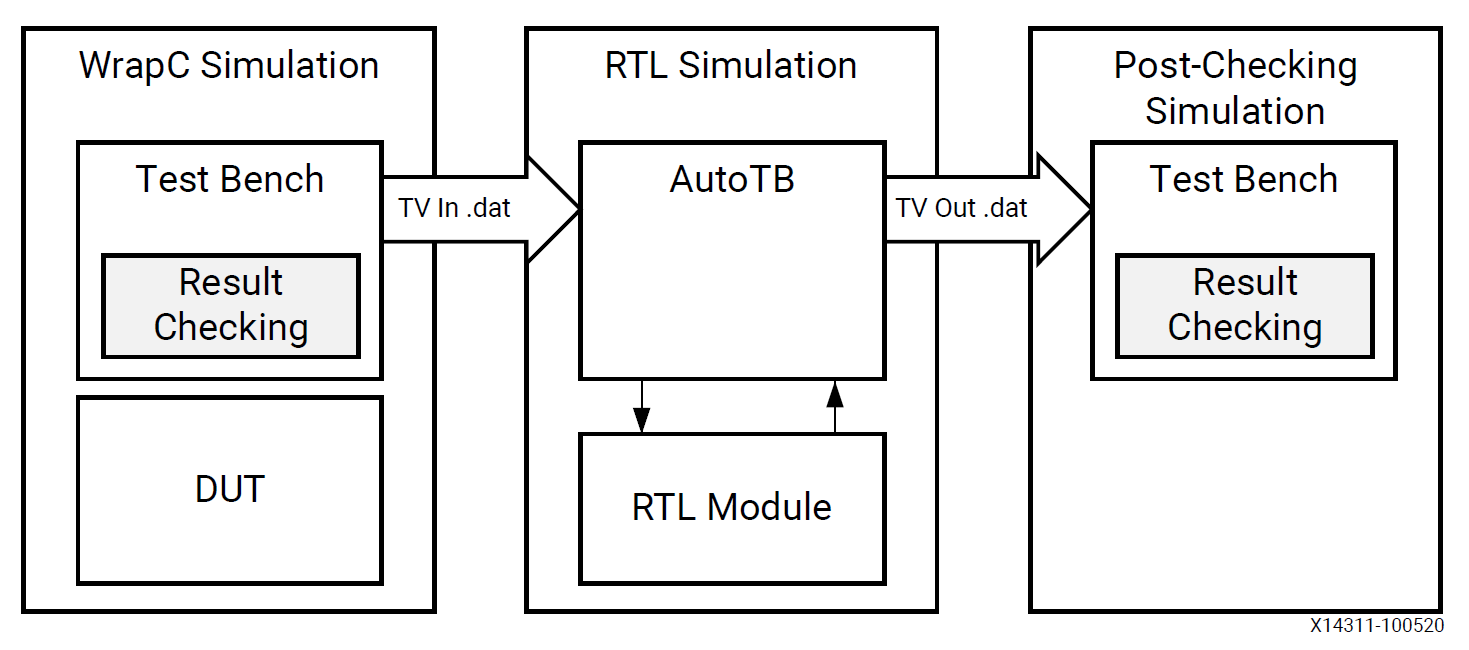
\includegraphics[width=0.9\textwidth]{images/CRTLVerification.PNG}
      \caption{C/RTL Verification Flow}
      \label{CRTLVerification.PNG}
  \end{center}
\end{figure}

C/RTL co-simulation uses a C test bench, running the main() function, to automatically verify the RTL design running in behavioral simulation. The C/RTL verification process consists of three phases:

\begin{enumerate}
  \item The C simulation is executed and the inputs to the top-level function, or the Design-Under-Test (DUT), are saved as "input vectors."
  \item The "input vectors" are used in an RTL simulation using the RTL created by Vitis HLS in Vivado simulator, or a supported third-party HDL simulator. The outputs from the RTL, or results of simulation, are saved as "output vectors."
  \item The "output vectors" from the RTL simulation are returned to the main() function of the C test bench to verify the results are correct. The C test bench performs verification of the results, in some cases by comparing to known good results.
\end{enumerate}

The following are requirements of C/RTL co-simulation:
\begin{itemize}
  \item The test bench must be self-checking as described in Writing a Test Bench, and return a value of 0 if the test passes or returns a non-zero value if the test fails.
  \item Any third-party simulators must be available in the search path to be launched by Vitis HLS.
  \item Interface Synthesis Requirements must be met (mentioned below).
  \item Any arrays or structs on the design interface cannot use the optimization directives listed in Unsupported Optimizations for Co-Simulation.
  \item IP simulation libraries must be compiled for use with third-party simulators as described in Simulating IP Cores.
\end{itemize}

Interface Synthesis Requirements: To use the C/RTL co-simulation feature to verify the RTL design, at least one of the following conditions must be true:
\begin{itemize}
  \item Top-level function must be synthesized using an ap\_ctrl\_chain or ap\_ctrl\_hs blocklevel protocol.
  \item Design must be purely combinational
  \item Top-level function must have an initiation interval of 1
  \item Interfaces must be all arrays that are streaming and implemented with axis or ap\_hs interface modes
\end{itemize}

\subsubsection{Verification of DATAFLOW and DEPENDENCE}
C/RTL co-simulation automatically verifies aspects of the DATAFLOW and DEPENDENCE directives. If the DATAFLOW directive is used to pipeline tasks, it inserts channels between the tasks to facilitate the flow of data between them. It is typical for the channels to be implemented with
FIFOs and the FIFO depth specified using the STREAM directive.

\par If co-simulation is attempted from the Vitis HLS IDE and the simulation results in a deadlock, the Vitis HLS IDE will automatically launch the Dataflow Viewer and show the processes involved in the deadlock (displayed in red). It will also show which channels are full (in red) versus empty (in white). 

\par In a similar manner, the RTL test bench is also configured to automatically check the validity of false dependencies specified using the DEPENDENCE directive. A warning message during cosimulation indicates the dependency is not false, and the corresponding directive must be removed to achieve a functionally valid design.

\subsubsection{Unsupported Optimizations for Co-Simulation}

For Vivado IP mode, automatic RTL verification does not support cases where multiple transformations are performed on arrays on the interface, or arrays within structs. In order for automatic verification to be performed, arrays on the function interface, or array inside structs on the function interface, can use any of the following optimizations, but not two or more:
\begin{itemize}
  \item Vertical mapping on arrays of the same size
  \item Reshape
  \item Partition, for dimension 1 of the array
\end{itemize}

Automatic RTL verification does not support any of the following optimizations used on a top-level function interface:
\begin{itemize}
  \item Horizontal mapping.
  \item Vertical mapping of arrays of different sizes.
  \item Conditional access on the AXI4-Stream with register slice enabled.
  \item Mapping arrays to streams.
\end{itemize}

\subsection{Analyzing RTL Simulations}
When the C/RTL co-simulation completes, the simulation report opens and  shows the measured latency and II. These results may differ from values reported after HLS synthesis. The results provided after C/RTL co-simulation show the actual values of latency and II for the given simulation data set (and may change if different input stimuli is used).

\par In non-pipelined designs, C/RTL co-simulation measures latency between ap\_start and ap\_done signals. The II is 1 more than the latency, because the design reads new inputs 1 cycle after all operations are complete.

\par In pipelined designs, the design might read new inputs before the first transaction completes, and there might be multiple ap\_start and ap\_ready signals before a transaction completes. In this case, C/RTL co-simulation measures the latency as the number of cycles between data input values and data output values. The II is the number of cycles between ap\_ready signals, which the design uses to requests new inputs.

\subsection{Cosim Deadlock Viewer}
A deadlock is a situation in which processes inside a DATAFLOW region share the same channels, effectively preventing each other from writing or reading from it, resulting in both processes getting stuck. This scenario is common when there are either FIFO's or a mix of PIPOs and FIFOs as channels inside the DATAFLOW.

\par The deadlock viewer visualizes this deadlock scenario on the static dataflow viewer. It highlights the problematic processes and channels. The viewer also provides a cross-probing capability to link between the problematic dataflow channels and the associated source code. The viewer automatically opens only after, the co-simulation detects the deadlock situation and the co-sim run has finished.

\subsection{Debugging C/RTL Co-Simulation}
When C/RTL co-simulation completes, Vitis HLS typically indicates that the simulations passed and the functionality of the RTL design matches the initial C code. 

\par Following are the primary reasons for a C/RTL co-simulation failure:
\begin{itemize}
  \item Incorrect environment setup
  \item Unsupported or incorrectly applied optimization directives
  \item Issues with the C test bench or the C source code
\end{itemize}

\section{Exporting the RTL Design}
The final step in the Vitis HLS flow is to export the RTL design in a form that can be used by other tools in the Xilinx design flow. When Vitis HLS reports the results of the high-level synthesis, it only provides an estimate of the results with projected clock frequencies and resource utilization (LUTs, DSPs, BRAMs, etc.). These results are only estimates because Vitis HLS cannot know what optimizations or routing delays will be in the final synthesized or implemented design. To get a better view of the RTL design, you can actually run Vivado synthesis and place and route on the generated RTL design, and review actual results of timing and resource utilization.

\clearpage
\section{Vitis HLS Command Line Interface}
Vitis HLS can be run from the GUI, interactively from the command line, or in batch mode from a Tcl script.

\subsection{Running Vitis HLS Interactively}
You can launch Vitis HLS using the -i option to open the tool in interactive mode.

\begin{lstlisting}[style=CStyle] 
  vitis_hls -i  // Launch Vitis HLS in interactive mode

  // The tool then displays a command line prompt
  vitis_hls> help // get a list of commands & Help for any command 

  // Vitis HLS supports an auto-complete feature by pressing the tab key
  exit // exit Vitis HLS.
  quit // quit Vitis HLS.
\end{lstlisting}

\subsection{Running Vitis HLS in Batch Mode}
Vitis HLS can also be run in batch mode, by specifying a Tcl script for the tool to run.

\begin{lstlisting}[style=CStyle]
  vitis_hls -f tcl_script.tcl  // Commands embedded in the specified 
  // script are executed in the specified sequence
\end{lstlisting}

If the Tcl script includes the exit or quit command, then the tool exits at that point, completing the batch process. If the Tcl script does not end with the exit command, Vitis HLS returns to the command prompt, letting you continue in interactive mode. All of the Tcl commands used when creating a project in the GUI are written to the solution/ script.tcl file within the project. You can use this script as a starting point for developing your own batch scripts. An example script is provided below:

\begin{lstlisting}[style=CStyle] 
  open_project dct
  set_top dct
  add_files ../dct_src/dct.cpp
  add_files -tb ../dct_src/out.golden.dat -cflags "-Wno-unknown-pragmas" -
  csimflags "-Wno-unknown-pragmas"
  add_files -tb ../dct_src/in.dat -cflags "-Wno-unknown-pragmas" -csimflags "-Wno-unknown-pragmas"
  add_files -tb ../dct_src/dct_test.cpp -cflags "-Wno-unknown-pragmas" -
  csimflags "-Wno-unknown-pragmas"
  open_solution "solution1" -flow_target vitis
  set_part {xcvu11p-flga2577-1-e}
  create_clock -period 10 -name default
  source "./dct/solution1/directives.tcl"
  csim_design
  csynth_design
  cosim_design
  export_design -format ip_catalog
\end{lstlisting}





% Chapter II Vitis HLS Hardware Design Methodology





\section{Designing Efficient Kernels}


\begin{highlight}
  Revisit  
\end{highlight}




\clearpage
\section{Vitis HLS Coding Styles}


This chapter explains how various constructs of C and C++11/C++14 are synthesized into an FPGA hardware implementation, and discusses any restrictions with regard to standard C coding.

The coding examples in this guide are available on GitHub for use with the Vitis HLS release. You can clone the examples repository from GitHub by clicking the Clone Examples command from the Vitis HLS Welcome screen.
Note: To view the Welcome screen at any time, select Help → Welcome.

\subsection{Unsupported C/C++ Constructs}
While Vitis HLS supports a wide range of the C/C++ languages, some constructs are not synthesizable, or can result in errors further down the design flow. To be synthesized:

\begin{itemize}
  \item The function must contain the entire functionality of the design.
  \item None of the functionality can be performed by system calls to the operating system.
  \item The C/C++ constructs must be of a fixed or bounded size.
  \item The implementation of those constructs must be unambiguous.
\end{itemize}

\subsubsection{System Calls}
System calls cannot be synthesized because they are actions that relate to performing some task upon the operating system in which the C/C++ program is running. Vitis HLS ignores commonly-used system calls that display only data and that have no impact on the execution of the algorithm, such as printf() and fprintf(stdout,). In general, calls to
the system cannot be synthesized and should be removed from the function before synthesis. Other examples of such calls are getc(), time(), sleep(), all of which make calls to the operating system.


\par Vitis HLS defines the macro \_\_SYNTHESIS\_\_ when synthesis is performed. This allows the \_\_SYNTHESIS\_\_ macro to exclude non-synthesizable code from the design.

\begin{highlight}
  Only the \_\_SYNTHESIS\_\_ macro should be used in the code to be synthesized. Macro in the test bench should not be used, as it is not obeyed by C/C++ simulation or C/C++ RTL co-simulation.
\end{highlight}

The \_\_SYNTHESIS\_\_ macro must not be defined or undefined in code or with compiler options, otherwise compilation might fail. The \_\_SYNTHESIS\_\_ macro is a convenient way to exclude non-synthesizable code without removing the code itself from the function, it can
result in different results between C/C++ simulation and C/C++ synthesis.

\subsubsection{Dynamic Memory Usage}
Any system calls that manage memory allocation within the system, for example, malloc(), alloc(), and free(), are not supported byt synthesis. Memory allocation system calls must be removed from the design code before synthesis. Xilinx recommends that you perform the following steps:

\begin{enumerate}[label=Step \arabic*:]
  \item Add the user-defined macro NO\_SYNTH to the code and modify the code.
  \item Enable macro NO\_SYNTH, execute the C/C++ simulation, and save the results.
  \item Disable the macro NO\_SYNTH, and execute the C/C++ simulation to verify that the results are identical.
  \item Perform synthesis with the user-defined macro disabled.
\end{enumerate}

This methodology ensures that the updated code is validated with C/C++ simulation and that the identical code is then synthesized.

\subsubsection{Pointer Limitations}
\begin{itemize}
  \item General Pointer Casting: Vitis HLS does not support general pointer casting, but supports pointer casting between native C/C++ types.
  \item Pointer Arrays: Vitis HLS supports pointer arrays for synthesis, provided that each pointer points to a scalar or an array of scalars. Arrays of pointers cannot point to additional pointers.
  \item Function Pointers: Function pointers are not supported.
  \item Pointer to pointer is not supported.
\end{itemize}

\subsubsection{Recursive Functions}
\begin{itemize}
  \item Recursive functions cannot be synthesized. This applies to functions that can form endless recursion.
  \item Vitis HLS also does not support tail recursion, in which there is a finite number of function calls.
  \item Virtual Functions are not supported.
\end{itemize}

\paragraph{Standard Template Libraries}
Many of the C++ Standard Template Libraries (STLs) contain function recursion and use dynamic memory allocation. For this reason, the STLs cannot be synthesized by Vitis HLS. The solution for STLs is to create a local function with identical functionality that does not feature recursion, dynamic memory allocation, or the dynamic creation and destruction of objects.

\subsection{Functions}
The top-level function becomes the top level of the RTL design after synthesis. Sub-functions are synthesized into blocks in the RTL design.

\begin{highlight}
  The top-level function cannot be a static function.
\end{highlight}

\subsubsection{Inlining Functions}
Sub-functions can optionally be inlined to merge their logic with the logic of the surrounding function. While inlining functions can result in better optimizations, it can also increase runtime as more logic must be kept in memory and analyzed.

\begin{highlight}
  Vitis HLS can perform automatic inlining of small functions.
\end{highlight} 

If a function is inlined, there is no report or separate RTL file for that function. The logic and loops of the sub-function are merged with the higher-level function in the hierarchy.

\subsubsection{C/C++ Builtin Functions}
Vitis HLS supports the following C/C++ builtin functions:
\begin{itemize}
  \item \_\_builtin\_clz(unsigned int x): Returns the number of leading 0-bits in x, starting at the most significant bit position. If x is 0, the result is undefined.
  \item \_\_builtin\_ctz(unsigned int x): Returns the number of trailing 0-bits in x, starting at the least significant bit position. If x is 0, the result is undefined.
\end{itemize}

\subsection{Loops}
Loops provide a very intuitive and concise way of capturing the behavior of an algorithm and are used often in C/C++ code. Loops are very well supported by synthesis. Loops can be pipelined, unrolled, partially unrolled, merged, and flattened.

\par The optimizations unroll, partially unroll, flatten, and merge effectively make changes to the loop structure as if the code were changed. These optimizations ensure that limited coding changes are required while optimizing the loops.

\begin{highlight}
  Avoid use of global variables for loop index variables, as this can inhibit some optimizations.
\end{highlight} 

The loop implementation techniques are as follows:
\begin{enumerate}
  \item Rolled implementation / iterative execution
  \item Full loop unroll
  \item Partial loop unroll
  \item Loop pipelining
\end{enumerate}

\subsubsection{Rolled implementation}
Rolled implementation or iterative execution is a default implementation. In rolled implementation, every iteration will execute in a serial and iterative manner. The loop will execute in 'n*k' cycles, where 'n' is number of loop iterations and 'k' is number of cycles required for each iteration. 
\begin{itemize}
  \item This type of implementation takes maximum time and minimum resources.
  \item The loops imply latency. Incrementing a loop counter always consumes at least one clock cycle.
  \item These rolled loops are treated as a single entity; all operations in the loop are implemented using the same hardware resources for each iteration of the loop.
\end{itemize}

\subsubsection{Full loop unroll}
In full loop unroll implementation, all the loops are removed by rewriting the operations of iterations of the loop. Loop becomes a basic block and schedule normally. This can be achieved using the following assumption:
\begin{highlight}
  There should not be any inter-iteration dependency, only then a full loop unroll can be achieved.
\end{highlight}

\begin{itemize}
  \item If a loop is completely unrolled, all operations will be performed in  parallel if data dependencies and resources allow. 
  \item In the fully unrolled version all loop operations can be performed in a single clock cycle.
  \item This type of implementation takes minimum time and maximum resources.
  \item Loops can be unrolled if their indices are statically determinable at elaboration time. They cannot be unrolled when the number of iterations is variable.
\end{itemize}

Syntax: \#pragma HLS UNROLL

\subsubsection{Partial loop unroll}
Partial loop unroll implementation is a tradeoff between Rolled implementation \& Full loop unroll implementation. In this implementation, the loop is unrolled by a certain factor provided by the designer.

\begin{highlight}
  As the loop is unrolled partially by a certain factor, the accesses/fetches from a memory are increased by the same factor. Hence, the array or memory must be split or partitioned.
\end{highlight}

Syntax: \#pragma HLS UNROLL factor=8

\begin{figure}[H]
	\begin{center}
		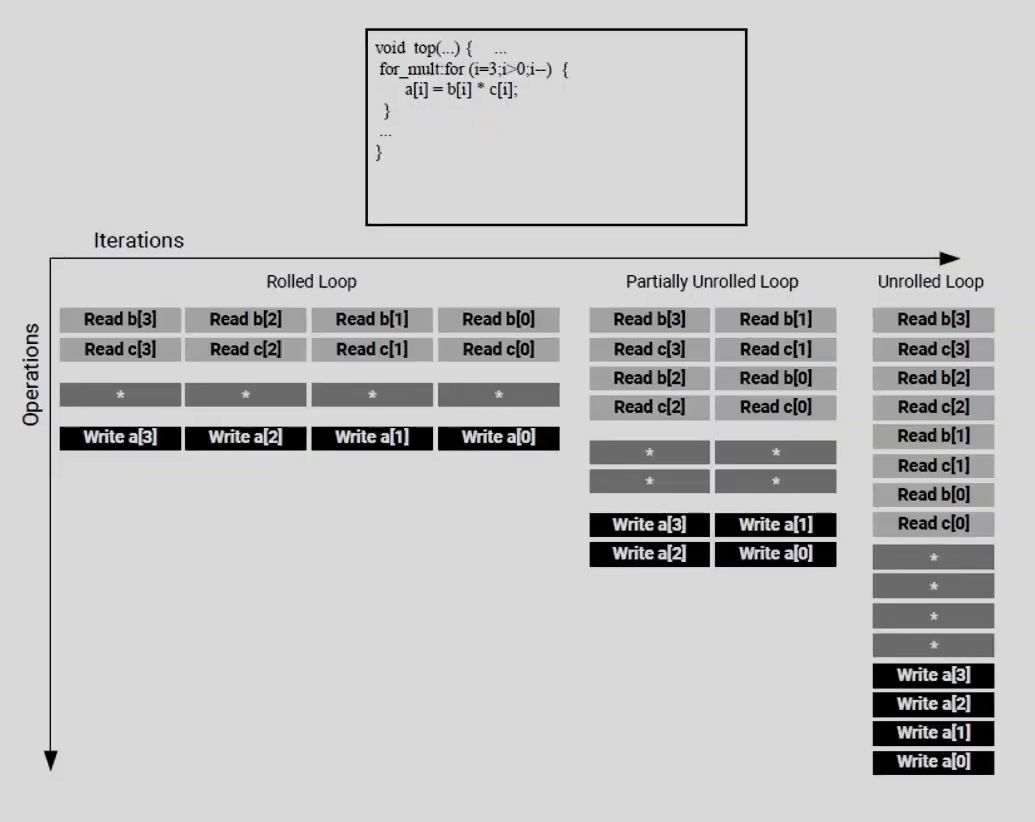
\includegraphics[width=\textwidth]{images/LoopRoll.png}
		\caption{Loop roll, unroll and partially unroll}
		\label{LoopRoll}
	\end{center}
\end{figure}

\subsubsection{Loop Pipelining}
Loop pipelining implementation allows the operations in a loop to be implemented in an overlapping manner. The pipeline executes until all iterations of the loop are completed.

\begin{figure}[H]
	\begin{center}
		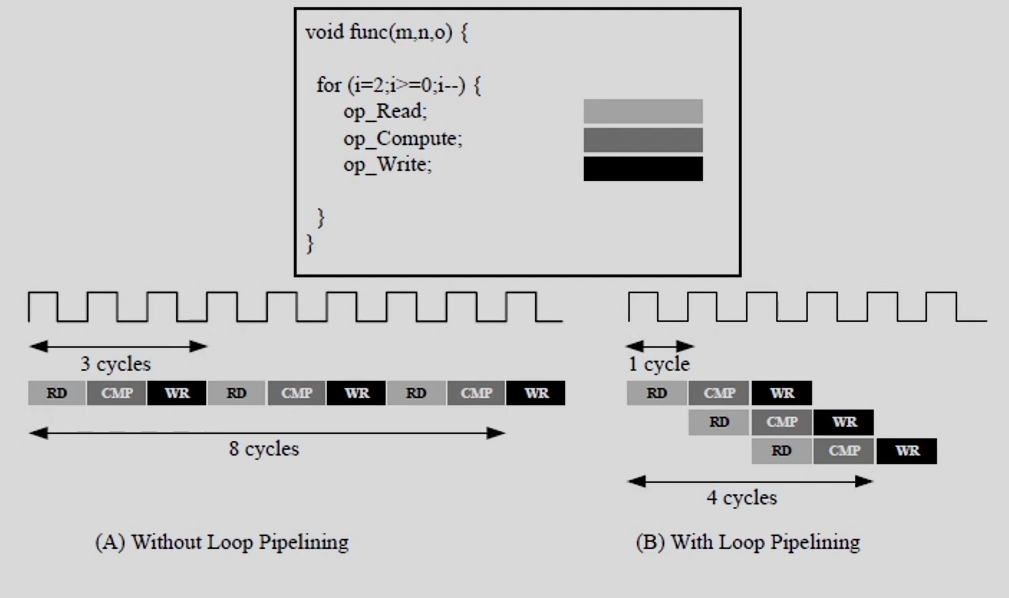
\includegraphics[width=\textwidth]{images/LoopPipe.png}
		\caption{Loop pipelining}
		\label{LoopPipe}
	\end{center}
\end{figure}

Syntax: \#pragma HLS PIPELINE II=1

\subsubsection{Nested Loop}
Having nested loops in C code is very common. In the case of nested loops:
\begin{itemize}
  \item Additional clock cycles are required to move between the rolled nested loops.
  \item One clock cycle is required to move from an outer loop to an inner loop and vice versa.
  \item When pipelining loops, the optimal balance between area and performance is typically found by pipelining the innermost loop. This also results in the fastest runtime.
  \item Pipelining the innermost loop gives the smallest hardware with generally acceptable throughput for most applications.
  \item When a loop or function is pipelined, any loop in the hierarchy below the loop or function being pipelined must be unrolled.
  \item There are three cases that can be explored: 
  \begin{enumerate}
    \item Pipelining the innermost loop (Minimum area, Good performance)
    \item Pipelining the outer loop and Unrolling the inner loop  (Low area, Better performance)
    \item Pipelining the function (Maximum area, Maximum performance)
  \end{enumerate}
\end{itemize}

The nested loops present in the code can be perfect, semi-perfect, or imperfect loops.
\begin{description}
  \item[Perfect Loops] In a perfect loop, only the innermost loop has the loop body content. There is no logic specified between the loop statements. All the loop bounds are constant.
  \item[Semi-Perfect Loops] In a semi-perfect loop, only the innermost loop has the loop body content. There is no logic specified between the loop statements. The outermost loop bound can be a variable.
  \item[Imperfect Loops] For imperfect loop nests where the inner loop has variable bounds or the loop body is not exclusively inside the inner loop, designers should try to restructure the code or unroll the loops in the loop body to create a perfect loop nest. The trivial transformation from an imperfect to perfect loop (initialization and
  final write) is made automatically by the tool. When the inner loop of a loop hierarchy is pipelined, Vitis HLS flattens the nested loops to reduce latency and improve overall throughput by removing any cycles caused by loop transitioning.
\end{description}

\subsubsection{Loop flattening}
The Vitis HLS tool provides the FLATTEN directive to allow the nested loops to be flattened, removing the need to recode for optimal hardware performance and reducing the number of cycles it takes to perform the operations in the loop.

\par The Vitis HLS tool can automatically flatten the nested loops. The recommendation is that the flattening should be specified on the innermost loop. The off option can prevent loops in the hierarchy from being flattened.

\subsubsection{Loop Merging}
Merging the loops allow the logic within the loops to be optimized together. It allows for more efficient architecture explorations.

All rolled loops imply and create at least one state in the design FSM. When there are multiple sequential loops, it can create additional unnecessary clock cycles and prevent further optimizations. The Vitis HLS tool provides the LOOP\_MERGE optimization directive, which can be
used to automatically merge the loops. The LOOP\_MERGE directive will seek to merge all the loops within the scope it is placed.


\paragraph{Loop Merging Rules}

Currently, the loop merging in the Vitis HLS tool has a few restrictions.
\begin{itemize}
  \item If loop bounds are all variables, they must have the same value.
  \item If loops bounds are constants, the maximum constant value is used as the bound of the merged loop.
  \item Loops with both variable bound and constant bound cannot be merged.
  \item Code between loops to be merged cannot have side effects: multiple execution of this code should generate the same results.
  \item Loops cannot be merged when they contain FIFO accesses. Merging would change the order of the reads and writes from a FIFO, which will affect the functioning of the FIFO.
  \item These loops can be merged using the force option.
\end{itemize}

\subsubsection{Variable Loop Bounds}
Some of the optimizations that Vitis HLS can apply are prevented when the loop has variable bounds. In this case, Vitis HLS cannot know when the loop will complete. Issues created by variable loop bounds are:

\begin{itemize}
  \item Variable loop bounds prevent Vitis HLS from determining the latency of the loop as Vitis HLS cannot statically determine the exact value of variable width, and hence, does not know the number of cycles to completely execute every iteration of the loop. Hence, variable bound loops cannot be unrolled.
  \item Another issue with variable loop bounds is that the performance of the design is unknown. There are two ways to overcome this issue: \begin{itemize}
    \item Use the pragma HLS loop\_tripcount or set\_directive\_loop\_tripcount. The tripcount is the number of loop iterations. The tripcount directive allows a minimum and/or maximum tripcount to be specified for the loop. 
    \item Use an assert macro in the C/C++ code.
  \end{itemize}  
\end{itemize}

The solution to loops with variable bounds is to make the number of loop iteration a fixed value with conditional executions inside the loop. \eg

\begin{lstlisting}[style=CStyle]
    #define N 32
    LOOP_X:for (x=0; x<N; x++) {
    if (x<width) {
    out_accum += A[x];
    }
    }
\end{lstlisting}

\subsubsection{Loop Parallelism}
Loop Parallelism refers to executing multiple loops parallely on the FPGA. Vitis HLS schedules logic and functions early as possible to reduce latency while keeping the estimated clock period below the user-specified period. To perform this, it schedules as many logic operations and functions as possible in parallel. 

\begin{itemize}
  \item Vitis HLS does not schedule loops to execute in parallel.
  \item If the loops have different bounds with same functionality, they cannot be merged. But, by placing the loops in separate functions, the identical functionality can be achieved and both loops can be scheduled in parallel as well.
  \item The principle of capturing loops in functions to exploit parallelism is presented here for cases in which dataflow optimization cannot be used.
  \item The dataflow optimization could also be used in the sequential loops.
\end{itemize}

\subsubsection{Loop Dependencies}
Loop dependencies are data dependencies that prevent optimization of loops, typically pipelining. They can be within a single iteration of a loop and or between different iteration of a loop. Loop dependencies can occur with any and all types of data. They are particularly common when
using arrays.

\subsection{Arrays}
\begin{itemize}
  \item Array is a contiguous memory. 
  \item Arrays are usually implemented as memory \ie RAM, ROM , or Registers. 
  \item Arrays on the top-level function interface are synthesized as RTL ports that access a memory outside.
  \item Internal to the design, arrays sized less than 1024 will be synthesized as FIFO. Arrays sized greater than 1024 will be synthesized into block RAM, LUTRAM, and UltraRAM depending on the optimization settings.
  \item Array access may create a bottleneck to performance. 
  \item These memories are accessed through ports. There are only a fixed number of ports(typically one or two)
\end{itemize}

\subsubsection{Minimize the parallel array access}
To mitigate this bottleneck, the designer has to minimize the parallel array access. It can be done in two ways: 
\begin{enumerate}
  \item Rewriting code to reduce memory access.
  \item Using HLS tool features to reduce the number of arrays.
\end{enumerate}

\paragraph{Rewriting code to reduce memory access}
\begin{itemize}
  \item Read array in minimum time
  \item Store locally and reuse
  \item Reduce memory access as much as possible 
\end{itemize}

\subsubsection{Array merging}
\begin{itemize}
  \item For multiple small arrays, there will be wastage of memory if we map each array to a RAM. 
  \item Small arrays can be merged into single block RAM.
  \item These small arrays should preferably have non-overlapping access.
  \item Merging can be done either horizontally or vertically. Extra locations in the memory will be padded with zeros.
  \item Syntax: \eg \#pragma HLS ARRAY\_MAP variable instance horizontal/vertical
\end{itemize}


\subsubsection{Array partitioning}
\begin{itemize}
  \item An array to be used will be larger than standard RAM size or it has many accesses.
  \item An array can be partitioned into multiple smaller arrays if it has non-overlapping accesses.
  \item Syntax: \eg \#pragma HLS array\_partition variable=<name> <type> factor=<int> dim=<int>
  
  \begin{itemize}
    \item Partition types: \begin{enumerate}
      \item Cyclic: cyclic partitioning creates smaller arrays by interleaving elements from the original array. 
      \item Block: block partitioning creates smaller arrays from blocks of the original array. This effectively splits the array into N equal blocks.
      \item Complete: complete partitioning decomposes the array into individual elements.
    \end{enumerate}
    \item factor: specifies the number of smaller arrays that are to be created.
    \item dim: specifies which dimension of a multi-dimensional array to partition.
  \end{itemize}
  \item Advantages of array partitioning: 
  \begin{itemize}
    \item Results in RTL with multiple small memories instead of one large memory.
    \item Effectively increases the amount of read and write ports for storage.
    \item Potentially improves the throughput of the design.
  \end{itemize}
\end{itemize}

\begin{figure}[H]
	\begin{center}
		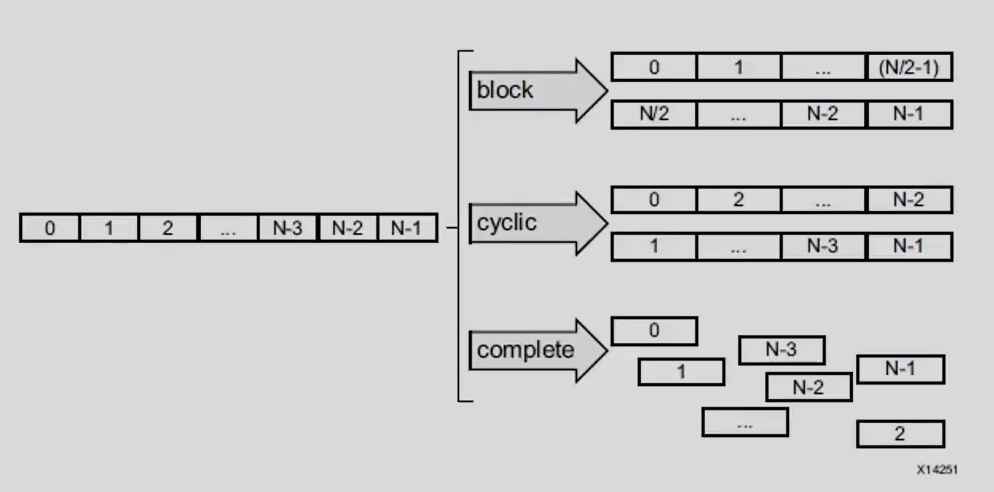
\includegraphics[width=\textwidth]{images/ArrayPart.png}
		\caption{Array partitioning}
		\label{ArrayPart}
	\end{center}
\end{figure}

\section{Defining Interfaces}
\section{Optimization Techniques in Vitis HLS}




  \clearpage

  \chapter{Vivado High-Level Synthesis Tutorial}   
  %  --------------------------------------------------  Lectures by Mirafra -------------------------------------------
The following tutorials explain and demonstrate all
steps in the process of transforming C, C++ and SystemC code to an RTL implementation
using High-Level Synthesis. These show how to create an initial RTL implementation
and then transform it into both a low-area and high-throughput implementation by
using optimization directives without changing the C code. 

\begin{highlight}
Reference for this sections: Vivado Design Suite Tutorial High-Level Synthesis UG871
\end{highlight}


\section{High-Level Synthesis Introduction}
This tutorial introduces Vivado High-Level Synthesis (HLS). The primary
tasks for performing High-Level Synthesis using both the Graphical User Interface (GUI) and
Tcl environments are demonstrated.

\subsection{Lab 1: Creating a High-Level Synthesis Project}
This lab explains how to set up a High-Level Synthesis (HLS) project and perform all the major steps in the HLS design flow:

\begin{enumerate}[label=Step \arabic*:]
    \item Creating a New Project: 
    \begin{enumerate}
        \item Open HLS GUI
        \item Enter project details (Name, Location)
        \item Add source files
        \item Add test bench files
        \item Generate Solution (specify hardware details \eg clock period, FPGA part, clock uncertainty)
    \end{enumerate}    
    \item Validate the C code (C Validation or C Simulation):\\
    Aim of this step is to confirm that the C code is correct. This process is also called {\bf C Validation or C Simulation.}
    \item High-Level Synthesis:\\ Synthesize the C design into an RTL design and review the synthesis report.
    \item RTL Verification:\\ High-Level Synthesis can re-use the C test bench to verify the RTL using simulation.
    \item IP Creation:\\ To package the design as an IP block for
    use with other tools in the Vivado Design Suite.
\end{enumerate}


\subsubsection{HLS Graphical User Interface (GUI)} 
Regions in the Graphical User Interface (GUI) and their functions are:
\begin{figure}[H]
    \begin{center}
        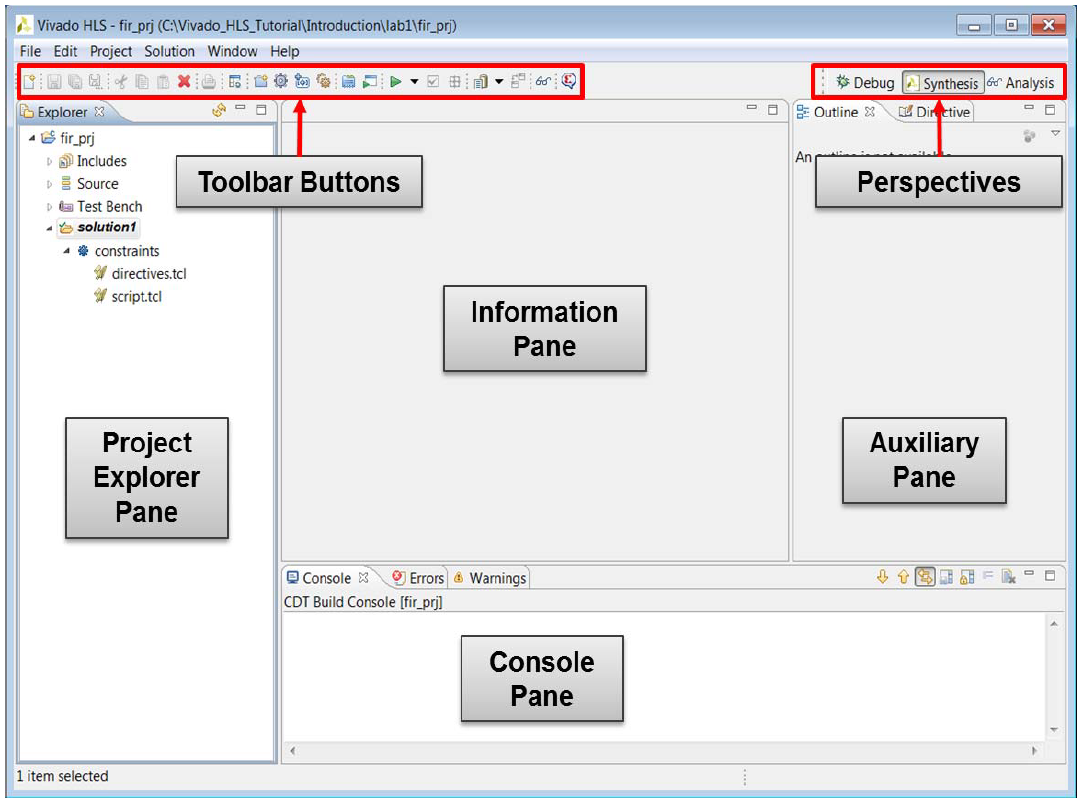
\includegraphics[width=0.8\textwidth]{images/panes.png}
        \caption{Vivado HLS Graphical User Interface}
        \label{panes}
    \end{center}
  \end{figure}

\begin{description}
    \item[Explorer Pane] Shows the project hierarchy.
    \item[Information Pane] Shows the contents of any files opened from the Explorer pane along with report files.
    \item[Auxiliary Pane] Cross-links with the Information pane.
    \item[Console Pane] Shows the messages produced when Vivado HLS runs. Errors and warnings appear in Console pane tabs.
    \item[Toolbar Buttons] Each button also has an associated menu item available from the pull-down menus to perform the most common operations.
    When you hold the cursor over the button, a popup tool tip opens, explaining the function.
    \item[Perspectives] Provide convenient ways to adjust the windows within the Vivado HLS GUI. 
    \begin{description}
        \item[Synthesis Perspective] The default perspective allows you to synthesize designs, run simulations, and package the IP.
        \item[Debug Perspective] Includes panes associated with debugging the C code.
        \item[Analysis Perspective] Windows in this perspective are configured to support analysis of synthesis results.
    \end{description}
\end{description}

\subsubsection{Usual self check operation of test bench}
\begin{itemize}
    \item The test bench saves the output in a file.
    \item That file is compared with the expected results stored in file.
    \item If the output matches the expected results, the return value of the test bench main() is set to 0. Else, the
    return value of main() is set to 1.
    \item If the test bench is self-checking, then the RTL results
    are automatically checked during RTL verification.
    \item The Vivado HLS tool can reuse the C test bench to perform verification of the RTL.
    \item There is no requirement to create an RTL test bench. This
    provides a robust and productive verification methodology.
\end{itemize}

\subsubsection{C synthesis report}
\begin{itemize}
    \item If the total latency is one clock cycle greater than the loop latency then,this indicates that the design is not pipelined.
    \item Vivado HLS targets a clock period of Clock Target minus Clock Uncertainty.
\end{itemize}

\begin{description}
    \item[Performance Estimates pane] 
    Performance Estimates pane enlists clock period, clock uncertainty, latency, Initiation Interval.
    \item[Utilization Estimates pane]
    Utilization Estimates pane tries to estimate the resource utilization numbers. These estimations might change post RTL synthesis with additional optimizations.
    \item[Interface pane] The Interface section shows the ports and I/O protocols created by interface synthesis. HLS automatically adds a clock and reset port along with a few interface ports.
\end{description}

\subsubsection{RTL co-simulation}
The default option for RTL co-simulation is to perform the simulation using the Vivado simulator and Verilog RTL. 

\subsection{Lab 2: Using the Tcl Command Interface}
This lab exercise shows how to create a Tcl command file based on an existing Vivado HLS project and use the Tcl interface:

\begin{enumerate}[label=Step \arabic*:]
    \item Open the Vivado HLS Command Prompt
    \item Generate a tcl file (For reference: Lab1 script.tcl)
    \item Run {\bf "vivado\_hls –f run\_hls.tcl"} in the the Vivado HLS Command Prompt (within required directory).
\end{enumerate}

\subsubsection{Important points to note}
\begin{itemize}
    \item When a Vivado HLS project is created, Tcl files(script.tcl \& directives.tcl) are automatically generated in the project hierarchy.
    \item The file script.tcl contains the Tcl commands to create a project with the files specified during the project setup and run all stages of the HLS flow.
    \item The file directives.tcl contains any optimizations applied to the design solution.
\end{itemize}
 
\subsection{Lab 3: Using Solutions for Design Optimization}
This lab shows you how to optimize the design using optimization directives. It also creates multiple versions of the RTL implementation and compares the different solutions.

\par Design goals:
\begin{itemize}
    \item Create a version of this design with the highest throughput.
    \item The final design should be able to process data supplied with an input valid signal.
    \item Produce output data accompanied by an output valid signal.
    \item The filter coefficients are to be stored externally to the FIR design, in a single port RAM.
\end{itemize} 

\begin{enumerate}[label=Step \arabic*:]
    \item Creating a New Project.    
    \item Optimize the I/O Interfaces:\\ The type of I/O protocol affects
    the design optimizations possibilities. Add directives from the Auxiliary Pane. Create multiple solutions with different optimizations.
    \item Analyze the Results:\\ Using Analysis perspective, performance and resources can be observed, analyzed. 
    \item Optimize for the Highest Throughput (Lowest Interval):\\ Unroll rolled, partition block RAM into individual registers.
    \item Compare the results of different solutions.
\end{enumerate}

\begin{itemize}
    \item If there is an I/O protocol requirement, setting the I/O protocol should be done as early as possible in the design cycle.
    \item Control states are the internal states High-Level Synthesis uses to schedule operations into clock cycles. There is a close
    correlation between the control states and the final states in the RTL Finite State Machine (FSM), but there is no one-to-one mapping.
    \item With the insight gained through analysis, you can proceed to optimize the design.
\end{itemize}

The two issues that limit the throughput are:
\begin{itemize}
    \item Rolled loops
    \item Use of block RAM instead of a shift-register
\end{itemize}


\section{C Validation}
Validation of the C algorithm is an important part of the High-Level Synthesis (HLS) process.
The time spent ensuring the C algorithm is performing the correct operation and creating
a C test bench, which confirms the results are correct, reduces the time spent analyzing
designs that are incorrect “by design” and ensures the RTL verification can be performed
automatically.

The sample design used in this tutorial is a Hamming Window FIR. There are three versions
of this design:
\begin{itemize}
    \item Using native C data types.
    \item Using ANSI C arbitrary precision data types.
    \item Using C++ arbitrary precision data types.
\end{itemize}
There are no design goals for this tutorial.


\subsection{Lab 1: C Validation and Debug}
Reviews the aspects of a good C test bench, the basic operations for C validation and the C debugger.

\begin{enumerate}[label=Step \arabic*:]
    \item Creating a New Project.    
    \item Review Test Bench and Run C Simulation
    \item Run the C Debugger
\end{enumerate}

\subsubsection{Good practices for writing a testbench}
\begin{itemize}
    \item The test bench creates and stores a set of expected results that confirm the function is correct.
    \item The test bench asks the Design Under Test (DUT) to generate and store results.
    \item The actual and expected results are compared. If the comparison fails, the value of variable err\_cnt is set to a non-zero value.
    \item The test bench issues a message to the console if the comparison failed, but more importantly returns the results of the comparison. 
    \item This process of checking the results and returning a value of zero if they are correct automates RTL verification.
\end{itemize}

\subsection{Lab 2: C Validation with ANSI C Arbitrary Precision Types}
Uses a design with arbitrary precision C types for C Validation.

\begin{enumerate}[label=Step \arabic*:]
    \item Creating a New Project
    \item Run the C Debugger with Launch Debugger:\\ Simulation is not completed as arbitrary precision types are not supported in debug mode.
    \item Run the C Debugger without Launch Debugger:\\ Run is successful.
\end{enumerate}

\begin{highlight}
    IMPORTANT: When working with arbitrary precision types you can use the Vivado HLS debug
    environment only with C++ or SystemC. When using arbitrary precision types with ANSI C,the debug
    environment cannot be used. With ANSI C, you must instead use printf or fprintf statements for
    debugging.    
\end{highlight}
 

\subsection{Lab 3: C Validation with C++ Arbitrary Precision Types}
Uses a design with arbitrary precision C++ types for C Validation.

\begin{enumerate}[label=Step \arabic*:]
    \item Creating a New Project
    \item Run the C Debugger with Launch Debugger:\\ Debugger is used to observe the arbitrary precision types being populated and utilized.
\end{enumerate}

\begin{highlight}
    Arbitrary precision types are a powerful means to create high-performance, bit accurate hardware designs. 
\end{highlight}



\section{Interface synthesis} 
Interface synthesis is the process of adding RTL ports to the C design. In addition to adding the physical ports to the RTL design, interface synthesis includes an associated I/O protocol, allowing the data transfer through the port to be synchronized automatically and optimally with the internal logic.


\subsection{Lab 1: Block-Level I/O Protocols}
Review the function return and block-level protocols. 


\begin{enumerate}[label=Step \arabic*:]
    \item Creating a New Project
    \item Create and Review the Default Block-Level I/O Protocol 
    \item Modify the Block-Level I/O protocol
\end{enumerate}

\subsubsection{Important points to be noted}
\begin{itemize}
    \item A clock and reset (single-bit inputs) have been added to the design by HLS.
    \item A block-level I/O protocol has been added to control the RTL design.
\end{itemize}

\subsubsection{Block level I/O Protocol}
The block-level I/O protocol allows the RTL design to be controlled by additional ports independently of the data I/O ports. This I/O protocol is associated with the function itself and not with any of the data ports. The default block-level I/O protocol is called ap\_ctrl\_hs (the Control Handshake protocol).

\par Behavior of the signals for block-level I/O protocol ap\_ctrl\_hs:
\begin{table}[H]
    \begin{center}    
    \begin{tabular}{|l|l|}
    \hline
    \textbf{Signal} &
      \textbf{Description} \\ \hline
    ap\_start &
      \begin{tabular}[c]{@{}l@{}}This signal controls the block execution and must be\\ asserted to logic 1 for the design to begin operation. \\ ap\_start should be held at logic 1 until the associated output\\ handshake ap\_ready is asserted. \end{tabular} \\ \hline
    ap\_ready &
      \begin{tabular}[c]{@{}l@{}}This output signal indicates when the design is ready for\\ new inputs. \end{tabular} \\ \hline
    ap\_done &
      \begin{tabular}[c]{@{}l@{}}This signal indicates when the design has completed all\\ operations in the current transaction.\end{tabular} \\ \hline
    ap\_idle &
      \begin{tabular}[c]{@{}l@{}}This signal indicates if the design is operating or idle (no\\ operation).\end{tabular} \\ \hline
    \end{tabular}
    \end{center}
\end{table}

\begin{itemize}
    \item The design does not start operation until ap\_start is set to logic 1.
    \item The design indicates it is no longer idle by setting port ap\_idle low.
    \item Output signal ap\_ready goes high to indicate the design is ready for new inputs on the next clock.
    \item Output signal ap\_done indicates when the design is finished and that the value on output port ap\_return is valid.
    \item If ap\_start is held high, the next transaction will start on the next clock cycle.
    \item In addition, the RTL cosimulation feature requires a block-level I/O protocol to sequence the test bench and RTL design for cosimulation automatically.
    \item {\it Cosim only supports the following 'ap\_ctrl\_none' designs: \begin{enumerate}
        \item Combinational designs
        \item Pipelined design with task interval of 1
        \item Designs with array streaming or hls\_stream ports
    \end{enumerate}
    }
\end{itemize}

\subsubsection{Types of the block-level interface protocol}
There are four types of the block-level interface protocol:

\begin{enumerate}
    \item ap\_ctrl\_none: No block-level I/O control protocol. When the interface protocol ap\_ctrl\_none is used, no block-level I/O protocols are added to the design. The only ports are those for the clock, reset and the data ports.
    \item ap\_ctrl\_hs: The block-level I/O control handshake protocol. This protocol is associated with the function return value (this is true even if the function has no return value specified in the code).
    \item ap\_ctrl\_chain: The block-level I/O protocol for control chaining. This I/O protocol is primarily used for chaining pipelined blocks together. In addition to the ap\_ctrl\_hs protocol but with an additional input signal, ap\_continue, which must be high when ap\_done is asserted for the next transaction to proceed. This
    allows downstream blocks to apply back-pressure on the system and halt further processing when they are unable to continue accepting new data.
    \item s\_axilite: Can be applied in addition to ap\_ctrl\_hs or ap\_ctrl\_chain to implement the block-level I/O protocol as an AXI Slave Lite interface in place of separate discrete I/O ports.
\end{enumerate}



\subsection{Lab 2: Port I/O Protocols}
Understand the default I/O protocol for ports and learn how to select an I/O protocol.

\begin{enumerate}[label=Step \arabic*:]
    \item Creating a New Project
    \item Specify the I/O Protocol for Ports
\end{enumerate}

\subsubsection{Important points to be noted}
\begin{itemize}
    \item The code does not have a function return, but instead passes the output of the function through the pointer argument. 
    \item The types of I/O protocol that you can add to C function arguments by interface synthesis
    depends on the argument type.

    \item Pass-by-value arguments can be implemented with the following I/O protocols:
    \begin{enumerate}
        \item ap\_none: No I/O protocol. This is the default for inputs.
        \item ap\_stable: No I/O protocol.
        \item ap\_ack: Implemented with an associated output acknowledge port.
        \item ap\_vld: Implemented with an associated input valid port.
        \item ap\_hs: Implemented with both input valid and output acknowledge ports.
    \end{enumerate}

    \item Pass-by-reference arguments that can be implemented with the following I/O protocols:
    \begin{enumerate}
        \item ap\_none: No I/O protocol. This is the default for inputs.
        \item ap\_stable: No I/O protocol.
        \item ap\_ack: Implemented with an associated input acknowledge port.
        \item ap\_vld: Implemented with an associated output valid port. This is the default for outputs.
        \item ap\_ovld: Implemented with an associated output valid port (no valid port for the input part of any inout ports).
        \item ap\_hs: Implemented with both input valid port and output acknowledge ports
        \item ap\_fifo: A FIFO interface with associated output write and input FIFO full ports.
        \item ap\_bus: A Vivado HLS bus interface protocol.
    \end{enumerate}
\end{itemize}

\subsection{Lab 3: Implementing Arrays as RTL Interfaces}
This lab reviews how array ports are implemented and can be partitioned.

\begin{enumerate}[label=Step \arabic*:]
    \item Creating a New Project (This design has an input array and an output array.)
    \item Synthesize Array Function Arguments to RAM Ports
    \item Using Dual-Port RAM and FIFO Interfaces
    \item Partitioned RAM and FIFO Array interfaces
    \item Fully Partitioned Array Interfaces
\end{enumerate}

\subsubsection{Important points to be noted}
\begin{itemize}
    \item Array arguments in the C source are by default synthesized into RTL RAM ports.
    \item High-Level Synthesis allows you to specify a RAM interface as a single-port or dual-port. If not specified, Vivado HLS automatically analyzes the design and selects the number of ports to maximize the data rate.
    \item An array argument is implemented using multiple RTL ports, only when the loops are unrolled or when the design is pipelined.
    \item By using a dual-port RAM interface, input data can be accepted at twice the rate as compared to a single-port RAM interface.
\end{itemize}

\subsection{Lab 4: Implementing AXI4 Interfaces}
Create an optimized implementation of the design and add AXI4 interfaces.

\begin{enumerate}[label=Step \arabic*:]
    \item Creating a New Project (This design has an input array and an output array.)
    \item Create an Optimized Design with AXI4-Stream Interfaces:\\ Varying the partitioning and loop unrolling allowed the optimal balance of area and performance.
    \item Implementing an AXI4-Lite Interfaces
\end{enumerate}

\begin{highlight}
    When AXI4-Lite interface is added, the IP packaging process creates software driver files to enable an external block, typically a CPU, to control this block (start, stop , set port values, review the interrupt status).
\end{highlight}


\section{Arbitrary Precision Types}
C/C++ provided data types are fixed to 8-bit boundaries:
\begin{itemize}
    \item char (8-bit)
    \item short (16-bit)
    \item int (32-bit)
    \item long long (64-bit)
    \item float (32-bit)
    \item double (64-bit)
    \item Exact width integer types such as int16\_t (16-bit) and int32\_t (32-bit)
\end{itemize}
Using standard C data types for
hardware design results in unnecessary hardware costs. Operations can use more LUTs and
registers than needed for the required accuracy, and delays might even exceed the clock
cycle, requiring more cycles to compute the result.

\begin{highlight}
    Vivado High-Level Synthesis (HLS) provides a number of bit accurate or arbitrary precision data-types, allowing you to model variables using any (arbitrary) width.
\end{highlight}

\subsection{Lab 1: Arbitrary Precision}
This lab synthesizes the same function used in Lab 1 using arbitrary precision fixed-types highlighting how the same design can be converted to the Vivado HLS ap\_fixed types, retaining the required accuracy but
creating a more optimal hardware implementation.

\begin{enumerate}[label=Step \arabic*:]
    \item Creating a New Project 
    \item Review Test Bench and Run C Simulation
    \item Synthesize the Design and Review Results
\end{enumerate}

\begin{highlight}
    High-Level Synthesis can synthesize floating-point types directly into hardware, provided the operations are standard arithmetic operations (+, -, *, \%).
\end{highlight}


\subsection{Lab 2: Arbitrary Precision}
This lab synthesizes a design using standard C++ floating-point types and reviews the results.

\begin{enumerate}[label=Step \arabic*:]
    \item Creating a New Project 
    \item Review Test Bench and Run C Simulation:\\ The test bench checks the accuracy of the results by comparing standard C++ floating-point types  with HLS Arbitrary Precision types. The results are within a specified range of accuracy.
    \item Synthesize the Design and Review Results:\\ Through use of arbitrary precision types, both the latency and
    the area have reduced (by 50\% and 80\% respectively), and the operations in the RTL hardware are no larger than necessary.
\end{enumerate}

\begin{highlight}
    Changing data types from standard C types to arbitrary precision types, make sure to reduce the size of the data types. This results in smaller operators, reduced area, and fewer clock cycles to complete.
\end{highlight}




\section{Design Analysis}
The general design methodology for creating an RTL implementation from C, C++, or SystemC includes the following tasks:
\begin{itemize}
    \item Synthesizing the design.
    \item Reviewing the results of the initial implementation.
    \item Applying optimization directives to improve performance.
\end{itemize}

These steps can be repeated until the required performance is achieved. Subsequently,the design can be revisited to improve area.

\begin{highlight}
    Vivado High-Level Synthesis (HLS) provides a number of bit accurate or arbitrary precision data-types, allowing you to model variables using any (arbitrary) width.
\end{highlight}

\subsection{Lab 1: Design Optimization}
This lab uses the insights from a DCT design analysis to applies optimizations and judges the effectiveness of the optimization.

\begin{enumerate}[label=Step \arabic*:]
    \item Creating a New Project 
    \item Review the Source Code and Create the Initial Design
    \item Review the Performance Using the Synthesis Report
    \item Review the Performance Using the Analysis Perspective
    \item Apply Loop Pipelining and Review for Loop Optimization
    \item Apply Loop Optimization and Review for Bottlenecks
    \item Partition Block RAMs and Analyze Concurrency
    \item Partition Block RAMs and Apply Dataflow optimization
    \item Optimize the Hierarchy for Dataflow
\end{enumerate}

\subsubsection{Important points to be noted}
\begin{itemize}
    \item High-level synthesis might automatically inline small functions to improve the quality of results (QoR). This can be prevented by adding the Inline directive with the -off option to any function being automatically inlined.
    \item The Analysis perspective consists of five panes: 
    \begin{itemize}
        \item Module Hierarchy Pane: Navigate through the hierarchy.
        \item Performance Profile Pane: the performance details for a particular level of hierarchy. Also shows how the operations in a particular block are scheduled into clock cycles.
        \item Resource Profile Pane: the resource details for a particular level of hierarchy.
        \item Console pane: Comprises of Properties, Outline, Warning, and C Source tab etc.
        \item Informtion pane: Shows the contents of any files opened along with report files.
    \end{itemize}
    \item To improve the initiation interval further from this state, 2 methods can be utilized:  
    \begin{itemize}
        \item Pipeline the loops
        \item Pipeline the entire function
    \end{itemize}
    \item Pipelining the function unrolls all the loops within it, and thus greatly increases the area. If the objective is to get the highest possible performance with no regard for area, this may be
    the best optimization to perform.
    \item Pipelining loops transforms the latency from\\
    Latency = iteration latency * (tripcount * interval)
    to\\
    Latency = iteration latency + (tripcount * interval)
    \item Bottlenecks are limitations in the flow of data that can
    prevent the logic blocks from working at their maximum data rate.
    Such limitations in the data flow can come from a number of sources.
    \item Another source of bottlenecks is data dependencies in the original source code. In some cases, these data dependencies are inherent in how the algorithm operates, as when a calculation cannot be performed until an earlier calculation has completed. Sometimes, however, the use of an optimization directive or a minor change to the C code can remove them.
    \item Approaches for identifying issues in the RTL design: 
    \begin{itemize}
        \item Start with the largest latency of interval in the Module Hierarchy report and navigate down the hierarchy to find the source of any large latency or interval.
        \item Click the Resource Profile to examine I/O and memory usage.
        \item With the use of graphical viewer, look for patterns in the Performance view which indicate a limitation in data flow.
    \end{itemize}
    \item The Resource view in analysis perspective shows how the resources in the design are used in different control states.
\end{itemize}



\section{Design Optimization}
A crucial part of creating high quality RTL designs using High-Level Synthesis is having the
ability to apply optimizations to the C code. High-Level Synthesis always tries to minimize
the latency of loops and functions.To achieve this, within the loops and functions, it tries to
execute as many operations as possible in parallel. At the level of functions, High-Level
Synthesis always tries to execute functions in parallel.

In addition to these automatic optimizations, directives are used to:
\begin{itemize}
    \item Execute multiple tasks in parallel, for example, multiple executions of the same function
    or multiple iterations of the same loop. This is pipelining.
    \item Restructure the physical implementation of arrays (block RAMs), functions, loops and
    ports to improve the availability of data and help data flow through the design faster.
    \item Provide information on data dependencies, or lack of them, allowing more
    optimizations to be performed.
\end{itemize}

The final optimization technique is to modify the C source code to remove unintended
dependencies in the code that may limit the performance of the hardware.

\subsection{Lab 1: Optimizing a Matrix Multiplier}

\subsubsection{Aim} To showcase contrast between the uses of loop and function pipelining to create a design that can process one sample per clock. To analyze loop
dependencies and data flow limitations or bottlenecks.

\par A matrix multiplier is used to design to show how to fully optimize a design
heavily based on loops. The design goal is to read one sample per clock cycle using a FIFO interface, while minimizing the area. 

\begin{enumerate}[label=Step \arabic*:]
    \item Create a project    
    \item Synthesize and Analyze the Design:\\ 
    By default, the code is implemented without pipelining to set the benchmark.
    \item Pipeline the Inner Loop:\\
    It fails to achieve the goal due to Carried dependency (mentioned below.)
    \item Pipeline the Outer Loop:\\ It fails to achieve the goal as 2-cycle BRAM read operations overlap.
    \item Reshape the Arrays:\\ Arrays are reshaped using Array Reshape Directive to achieve 1 clock cycle II.
    \item Apply FIFO Interfaces:\\ It is impossible to use a FIFO interface for data access with the code as written. To use a FIFO interface, the optimization directives available in Vivado HLS are inadequate as the code currently enforces a certain order of reads and writes.
    \item Pipeline the Function:\\ The design latency decreases further however, the area and resources have increased substantially as all the loops are unrolled.
\end{enumerate}

{\bf Important points to be noted:
\begin{itemize}
    \item To improve the initiation interval further from this state, 2 methods can be utilized: 
    \begin{itemize}
        \item Pipeline the loops
        \item Pipeline the entire function
    \end{itemize}
    \item When pipelining nested loops, pipelining the inner-most loop, might affect the highest as it is ran the most number of times. 
    \item Carried dependency: This is a dependency between an operation in one iteration of a loop and an operation in a different iteration of the same loop.
    \item High-Level Synthesis automatically applies loop flattening, collapsing the nested loops, removing the loop transitions (essentially creating a
    single loop with more iterations but overall fewer clock cycles).
    \item Arrays are implemented as block RAMs and arrays which are arguments to the function are implemented as block RAM ports. As a block RAM can only have a maximum of two ports (for dual-port block RAM), reading more than 2 values in one clock cycle is not possible.
    \item High-Level Synthesis allows arrays to be partitioned, mapped together and re-shaped.
    \item High-Level Synthesis can only report one schedule error or warning at a time.
    \item The default behavior of High-Level Synthesis is to produce a design with the
    highest performance.
    \item Pipelining loops allows the loops to remain rolled, thus providing a good means of
    controlling the area.
    \item The pipelined function results in the best performance.
    \item There is a trade off between Performance and Area.
\end{itemize}
}

\subsection{Lab 2: C Code Optimized for I/O Accesses}
This lab shows how modifications to the code can help overcome some performance limitations inherent, but unintended, in the code.

\par In lab 1, the nature of the C code, which specified multiple accesses to the same addresses, prevented streaming interfaces being applied.
\begin{itemize}
    \item In a streaming interface, the values must be accessed in sequential order.
    \item HLS cannot decide to change the specification of the algorithm.
\end{itemize}

\begin{enumerate}[label=Step \arabic*:]
    \item Create a project    
    \item Review the code:\\ 
    \begin{itemize}
        \item The directives are specified in the code as pragmas.
        \item For-loops have been added to cache the row and column reads.
        \item A temporary variable is used for the accumulation and result is written only when the final result is computed for each value.
        \item Cache for-loops are automatically unrolled.
    \end{itemize}
    \item Synthesize the design and verify the RTL using co-simulation:\\ Successful synthesis with reading one sample every clock cycle using streaming FIFO interfaces.
\end{enumerate}

\section{RTL Verification}
The High Level Synthesis tool automates the process of RTL verification and allows you to use RTL verification to generate trace files that show the activity of the waveforms in the RTL design. 

RTL verification is often called cosimulation or C/RTL cosimulation; as both C and RTL are used in the verification.

\subsection{Lab 1: RTL Verification and the C Test Bench}
This lab performs RTL verification steps and understands the importance of the C test bench in verifying the RTL.

\begin{enumerate}[label=Step \arabic*:]
    \item Create a project    
    \item Perform RTL Verification:\\ 
    \item Modify the C test bench
\end{enumerate}

\subsection{Lab 2: Viewing Trace Files in Vivado}
This lab creates RTL trace files and analyzes them using the Vivado Design Suite. The steps involved in the lab are:
\begin{enumerate}[label=Step \arabic*:]
    \item Create an RTL Trace File using Vivado Simulator.
    \item Perform RTL Verification
    \item Modify the C test bench
\end{enumerate}

RTL simulation comprises of three phases.
\begin{enumerate}[label=Phase \arabic*:]
    \item WrapC Simulation: The C test bench is executed to generate input stimuli for the RTL design.
    \item RTL Simulation: An RTL test bench with newly generated input stimuli is created and the RTL simulation is then performed.
    \item Post-Checking Simulation: Finally, the output from the RTL simulation is re-applied to the C test bench to check the results. 
\end{enumerate}
RTL verification issues message SIM-1000 if the RTL verification passed.

\subsection{Lab 3: Viewing Trace Files in ModelSim}
This lab creates RTL trace files and analyzes them using a third-party RTL simulator. 

\section{Using HLS IP in IP Integrator}
RTL from High-Level Synthesis can be packaged and use it inside IP Integrator.

\subsection{Lab 1: Integrate HLS IP with a Xilinx IP Block}
This lab completes the steps to generate two HLS blocks for the IP catalog and use them in a design with Xilinx IP, an FFT. The objective is to validate and verify the final design using an RTL test bench.

\begin{enumerate}[label=Step \arabic*:]
    \item Create Vivado HLS IP Blocks
    \item Create a Vivado Design Suite Project
    \item Add HLS IP to an IP Repository
    \item Create a Block Design for RealFFT
    \item Verify the Design
\end{enumerate}



\section{Using HLS IP in a Zynq AP SoC Design}
A common use of High-Level Synthesis design is to create an accelerator for a CPU – to move code that executes on the CPU into the FPGA programmable logic to improve performance. 

\subsection{Lab 1: Implement Vivado HLS IP on a Zynq Device}
This lab integrates both the High-Level Synthesis IP and the software drivers created by HLS to control the IP in a design implemented on a Zynq device.

\begin{enumerate}[label=Step \arabic*:]
    \item Create a Vivado HLS IP Block
    \item Create a Vivado Zynq Project
    \item Add HLS IP to the IP Catalog
    \item Creating an IP Integrator Block Design of the System
    \item Implementing the System
    \item Developing Software and Running it on the Zynq System
    \item Modify software to communicate with HLS block
\end{enumerate}

\subsection{Lab 2: Streaming Data Between the Zynq CPU and HLS Accelerator Blocks}
This lab illustrates a common high performance connection scheme for connecting hardware accelerator blocks that consume data originating in the CPU memory and/or producing data destined for it in a streaming manner. 
  \clearpage

  \chapter{References}
  \begin{itemize}     
    \item \href{https://www.xilinx.com/support/documentation/sw_manuals/xilinx2021_1/ug1399-vitis-hls.pdf}{Vitis High-Level Synthesis User Guide (UG1399)}
    \item \href{https://www.xilinx.com/support/documentation/sw_manuals/ug998-vivado-intro-fpga-design-hls.pdf}{Introduction to FPGA Design with Vivado High-Level Synthesis (UG998)}
    \item \href{https://www.xilinx.com/support/documentation/sw_manuals/xilinx2018_3/ug902-vivado-high-level-synthesis.pdf}{Vivado Design Suite User Guide High-Level Synthesis (UG902)}
    \item \href{https://www.xilinx.com/support/documentation/sw_manuals/xilinx2014_2/ug871-vivado-high-level-synthesis-tutorial.pdf}{Vivado Design Suite Tutorial High-Level Synthesis Tutorial (UG871)}
    \item \href{https://github.com/Xilinx/Vitis-Tutorials/tree/2021.1/Hardware_Acceleration}{Hardware Acceleration Labs Github}
    \item \href{https://www.xilinx.com/support/documentation/sw_manuals/xilinx2020_1/ug1391-vitis-hls-migration-guide.pdf}{Vitis HLS Migration Guide (UG1391)}
  \end{itemize}


	
\end{document}




